\chapter{Materiais e Métodos} \label{ch:materiais}
\setlength{\headheight}{13.6pt}
%%%%%%%%%%%%%%%%%%%%%%%%%%%%%%%%%%%%%%%%%%%%%%%%%%%%%%%%%%%%%%%%%%%%%%%%%%%%%
\section{Introdução} \label{sec:materiais_intro}
Como já foi referido, o principal objetivo deste trabalho é desenvolver uma ferramenta porta-peças para proteger o diâmetro interno das rodas de coroa \textbf{BD35}, \textbf{DB45} e \textbf{JT4}, de forma a melhorar a operação de torneamento duro e diminuir a ocorrência de não conformidades devidas à fissurações a frio. 
\par
Assim, este capítulo começa por descrever o \textbf{caso de estudo}, isto é, as rodas de coroa em que será feito o processo de carbonitruração e seu processo de maquinação antes deste processo(que é mencionado a seguir como “processo de obtenção da peça branca”), as ferramentas porta-peças atualmente utilizadas no processo de carbonitruração das rodas de coroa supracitadas(que a partir deste ponto são chamadas peças negras), e o processo de torneamento, onde é obtida a geometria final das rodas de coroa que posteriormente serão prensadas e soldadas à caixa diferencial.
\par
É então apresentado o processo de simulação por CFD que as rodas de coroa serão sujeitos, para a linha de série e para todas as soluções propostas, e em seguida, é apresentada uma solução inicial, chamada de \textbf{“Tampa P”}, simples, onde as únicas diferenças desta solução para a ferramenta atualmente utilizada são a modificação da \textit{falsa coroa} para não permitir a passagem de fluido \textbf{por baixo} e a adição de uma \textit{tampa} \textbf{em cima} com efeito análogo. Somado a isto, são apresentadas três soluções complementares, cujo objetivo é melhorar alguns parâmetros obtidos no ensaio da solução inicial \textbf{“P”}, no caso das tampas \textbf{“Y”} e \textbf{“O”}, ou simplificar o sistema, no caso da solução \textbf{“Sem tampa”}.
\par
Por fim, são descritos os \textbf{parâmetros de conformidade} e o processo de ensaio para verificação dos impactos das várias modificações, que posteriormente serão analisados e discutidos no capítulo \ref{ch:resultados}, e uma vez que estes serão utilizados para validar os parâmetros de conformidade, serão também apresentados os métodos de ensaio de dureza, de verificação dimensional e o ensaio de difusibilidade do hidrogénio.
\newpage
%%%%%%%%%%%%%%%%%%%%%%%%%%%%%%%%%%%%%%%%%%%%%%%%%%%%%%%%%%%%%%%%%%%%%%%%%%%%%
\section{Caso de estudo} \label{sec:materiais_CS}
\subsection{Processo de obtenção da peça branca} \label{ssec:materiais_CS_peca_branca}

O processo de produção da peça branca, inicia-se com um bruto de aço de baixa liga \textbf{AFNOR 27MC5}, ou \textbf{EN-1.7149}. Cada série de rodas de coroa tem um bruto de dimensões específicas, bem como programas de maquinação e padrões de conformidade específicos. Como exemplo, na Figura \ref{fig:Bruto_desenho} vê-se as dimensões do bruto das rodas de coroa DB45 de aproximadamente 204,4 mm de diâmetro externo, 106 mm de diâmetro interno e 39 mm de espessura.

%%%%%%%%%%%%%%%%%%%%%%%%%%%%%%%%%%%%%%%%%%%%%%%%%%%%%%%%%%%%%%%%%%%%%%%%%%%%%
\begin{figure}[htb]
    \centering
    \begin{subfigure}{.5\textwidth}
        \centering
        \includegraphics[width = 0.9\textwidth]{Figures/Cap3/Bruto_fotografia.png}
        \caption{}
        \label{fig:Bruto_fotografia}
    \end{subfigure}%
    \begin{subfigure}{.5\textwidth}
        \centering
        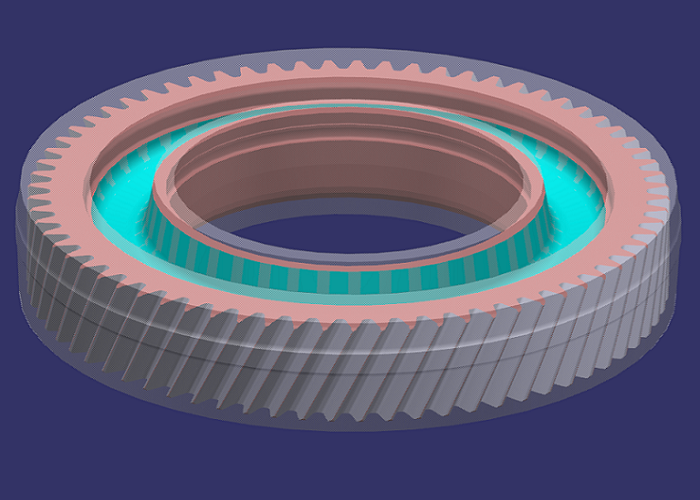
\includegraphics[width = 0.9\textwidth]{Figures/Cap3/Bruto_CAD.png}
        \caption{}
        \label{fig:Bruto_desenho}
    \end{subfigure}
    \caption[Imagens do bruto para fabricação da peça branca]%
    {À esquerda, uma fotografia de um bruto utilizado para obter a peça branca. À direita, um desenho com as dimensões do bruto e hachuras com o formato e dimensões da peça branca final.}
\end{figure}
%%%%%%%%%%%%%%%%%%%%%%%%%%%%%%%%%%%%%%%%%%%%%%%%%%%%%%%%%%%%%%%%%%%%%%%%%%%%%

\par
Deste bruto, serão removidos os excessos de material do diâmetro interno, das faces superior e inferior, e maquinado o dentado, tudo isto feito de forma automática, sendo apenas necessária a intervenção do operador na alimentação inicial dos brutos na linha de produção, na troca das ferramentas, seja por desgaste ou por mudança da série a maquinar, ou em casos de defeitos de máquina. Cada operação é realizada num centro de maquinagem diferente, e o transporte é realizado por meio de transportadores mecânicos, o que torna o processo mais ágil e permite a continuação do processo produtivo em caso de avaria de algum dos centros.

\par
Após estarem maquinadas as rodas de coroa, estas estão prontas para seguir para o processo de carbonitruração, processo que tornar-lhes-á peças negras. Portanto, após a saída do último centro de maquinagem, as rodas de coroa são direcionadas a uma ilha em que um braço mecânico carrega de forma ordenada uma carga, composta por três pratos de cinco colunas cada, totalizando quinze colunas por carga. O número de rodas de coroa por coluna varia entre 10, no caso das séries “DB45” e 11, no caso das séries “DB35” e “JT4”. Isto é devido ao peso máximo suportado pelo elevador do forno de carbonitruração, que tem um limite de 550kg. Sendo as séries “DB45” mais espessas, portanto, mais pesadas, existe a necessidade da redução do número de rodas de coroa de 55 para 50 por prato.
%%%%%%%%%%%%%%%%%%%%%%%%%%%%%%%%%%%%%%%%%%%%%%%%%%%%%%%%%%%%%%%%%%%%%%%%%%%%%
\begin{figure}[htb]
    \centering
    \begin{subfigure}{.45\textwidth}
        \centering
        \includegraphics[width = 0.9\textwidth]{Figures/Cap3/Peca_branca_fotografia.png}
        \caption[]%
        {}
        \label{fig:Peca_branca_fotografia}
    \end{subfigure}%
    \begin{subfigure}{.45\textwidth}
        \centering
        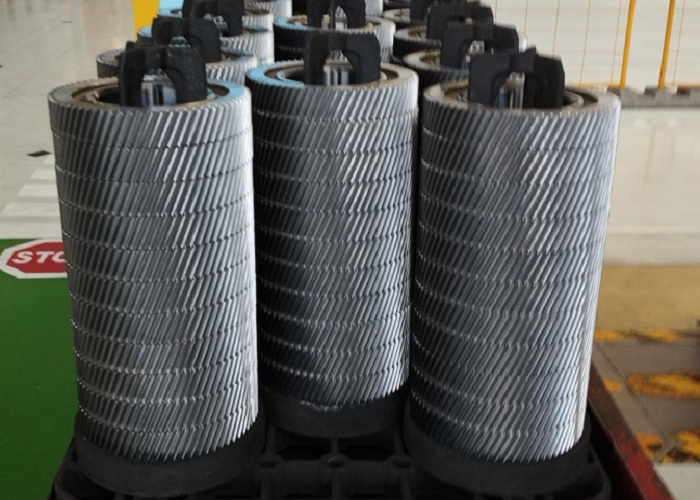
\includegraphics[width = 0.9\textwidth]{Figures/Cap3/Carga_fotografia.png}
        \caption{}
        \label{fig:Carga_peca_branca}
    \end{subfigure}
    \caption[Peça branca final e Prato de Rodas de coroa série DB35]%
    {À esquerda, uma fotografia de uma roda de coroa DB45 peça branca. À direita, uma fotografia de um prato montado com 50 rodas de coroa DB45 “peça branca” maquinadas.}
\end{figure}
%%%%%%%%%%%%%%%%%%%%%%%%%%%%%%%%%%%%%%%%%%%%%%%%%%%%%%%%%%%%%%%%%%%%%%%%%%%%%
\subsection{Processo de tratamentos térmicos} \label{ssec:materiais_CS_carbonitruracao}
Chegando a carga na zona dos tratamentos térmicos, esta é carregada para uma máquina de pré-oxidação, este processo precede a carbonitruração e é utilizado para melhorar a aderência da camada de carbono e azoto adquirida. Para uma melhor perceção do sistema, as Figuras \ref{fig:Prato}, \ref{fig:Torre} e \ref{fig:Falsa_coroa} ilustram as tres partes da ferramenta porta-peças atualmente utilizados em toda a linha dos tratamentos térmicos. O material dos componentes da ferramenta porta-peças é o \textbf{aço refratário EN 1.4807}.

%%%%%%%%%%%%%%%%%%%%%%%%%%%%%%%%%%%%%%%%%%%%%%%%%%%%%%%%%%%%%%%%%%%%%%%%%%%%%
\begin{figure}[htb]
    \centering
    \begin{subfigure}{.33\textwidth}\
        \centering
        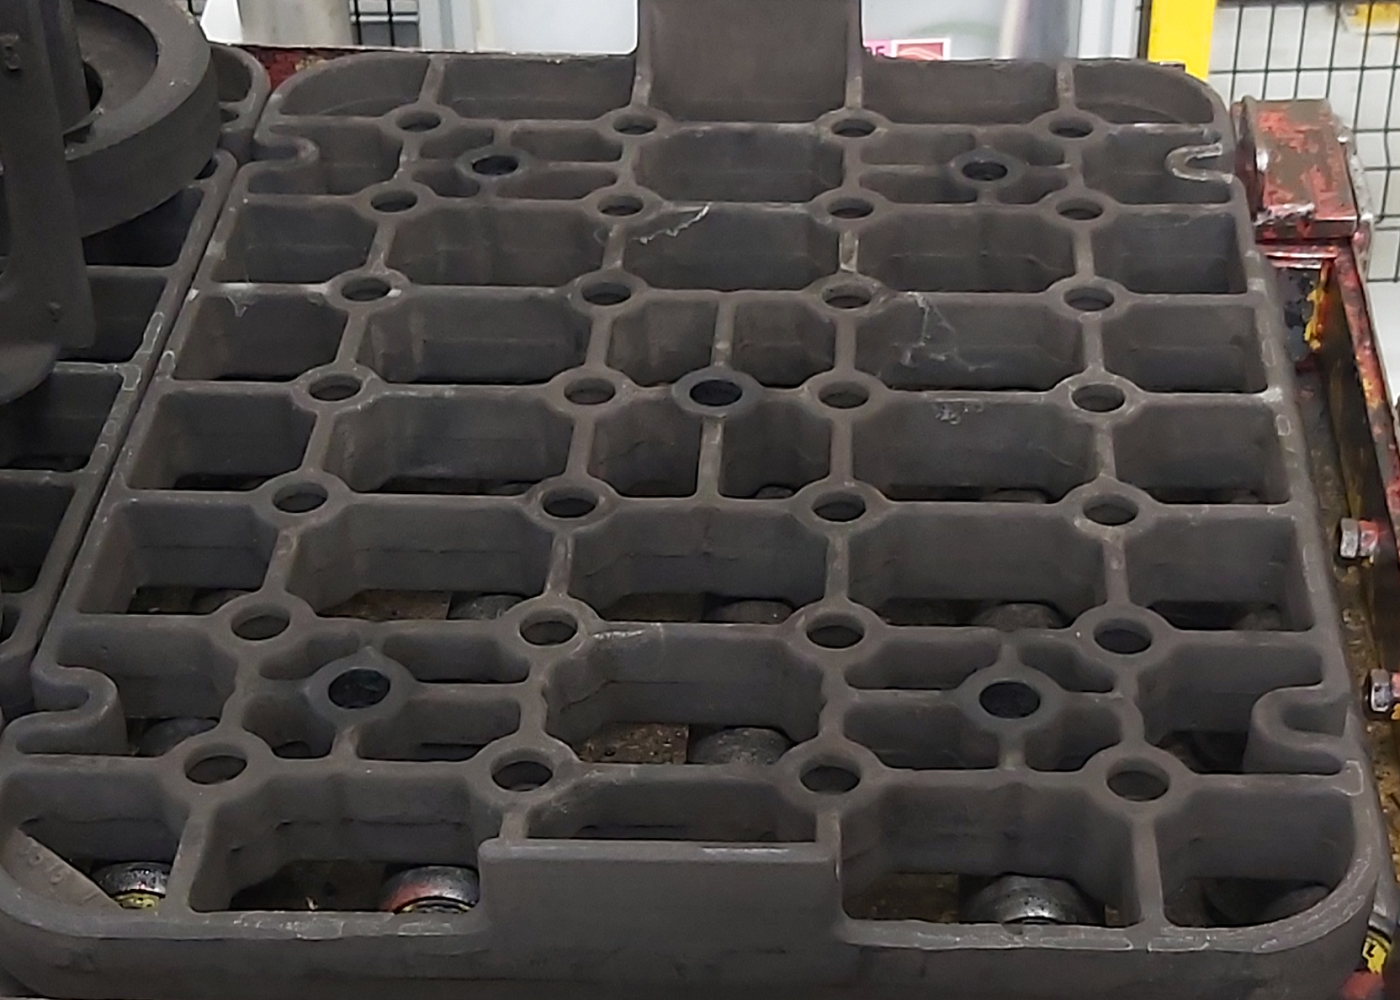
\includegraphics[width = 0.9\textwidth]{Figures/Cap3/Prato.png}
        \caption{}
        \label{fig:Prato}
    \end{subfigure}%
    \centering
    \begin{subfigure}{.33\textwidth}
        \centering
        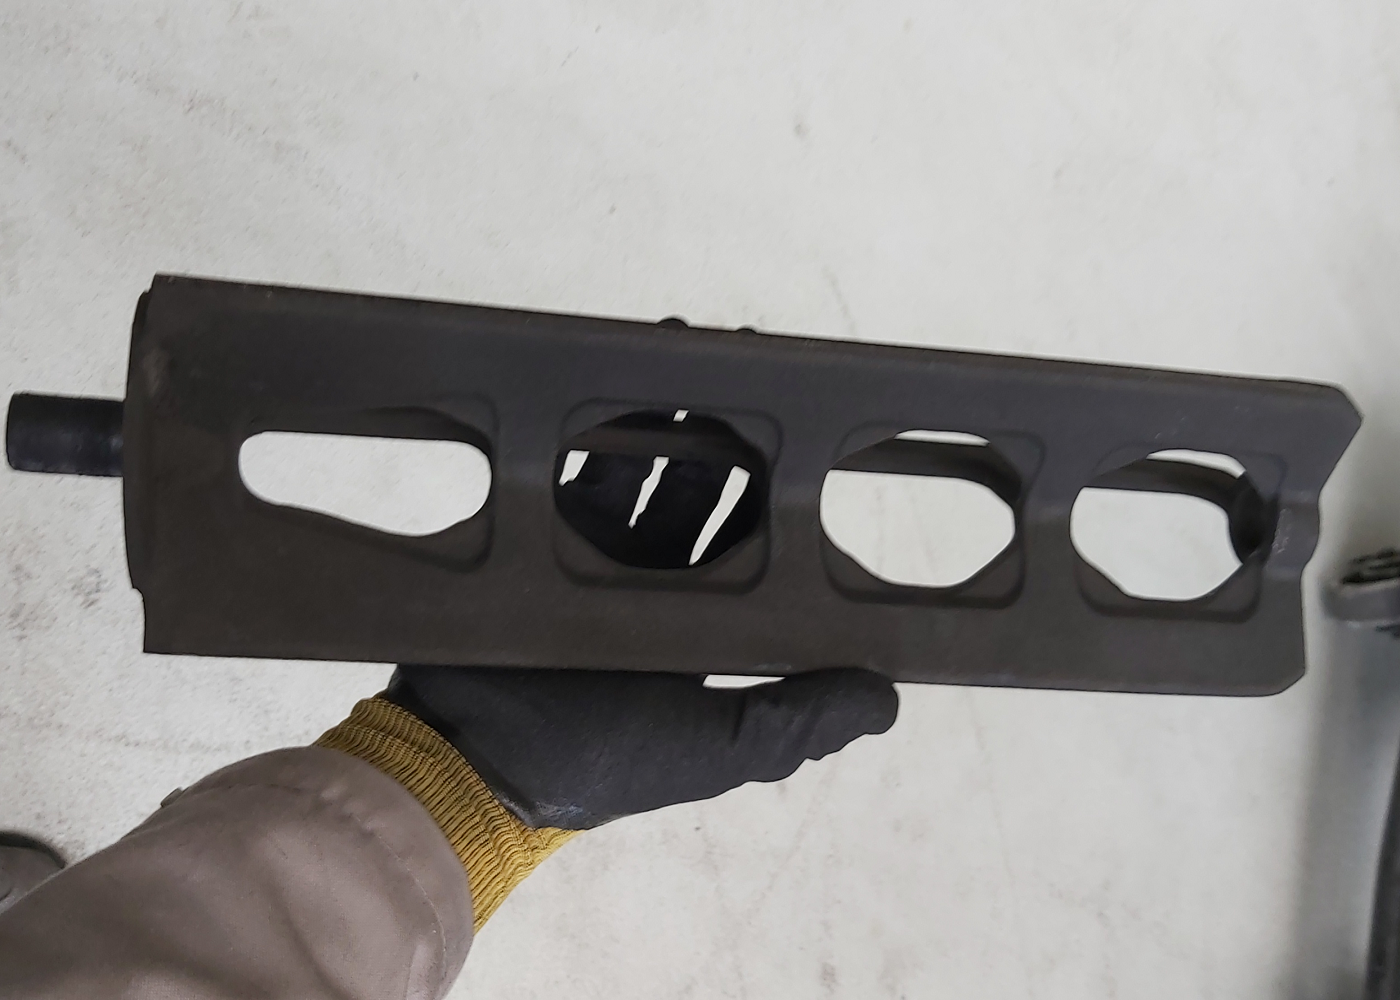
\includegraphics[width = 0.9\textwidth]{Figures/Cap3/Torre.png}
        \caption{}
        \label{fig:Torre}
    \end{subfigure}
    \centering
    \begin{subfigure}{.33\textwidth}
        \centering
        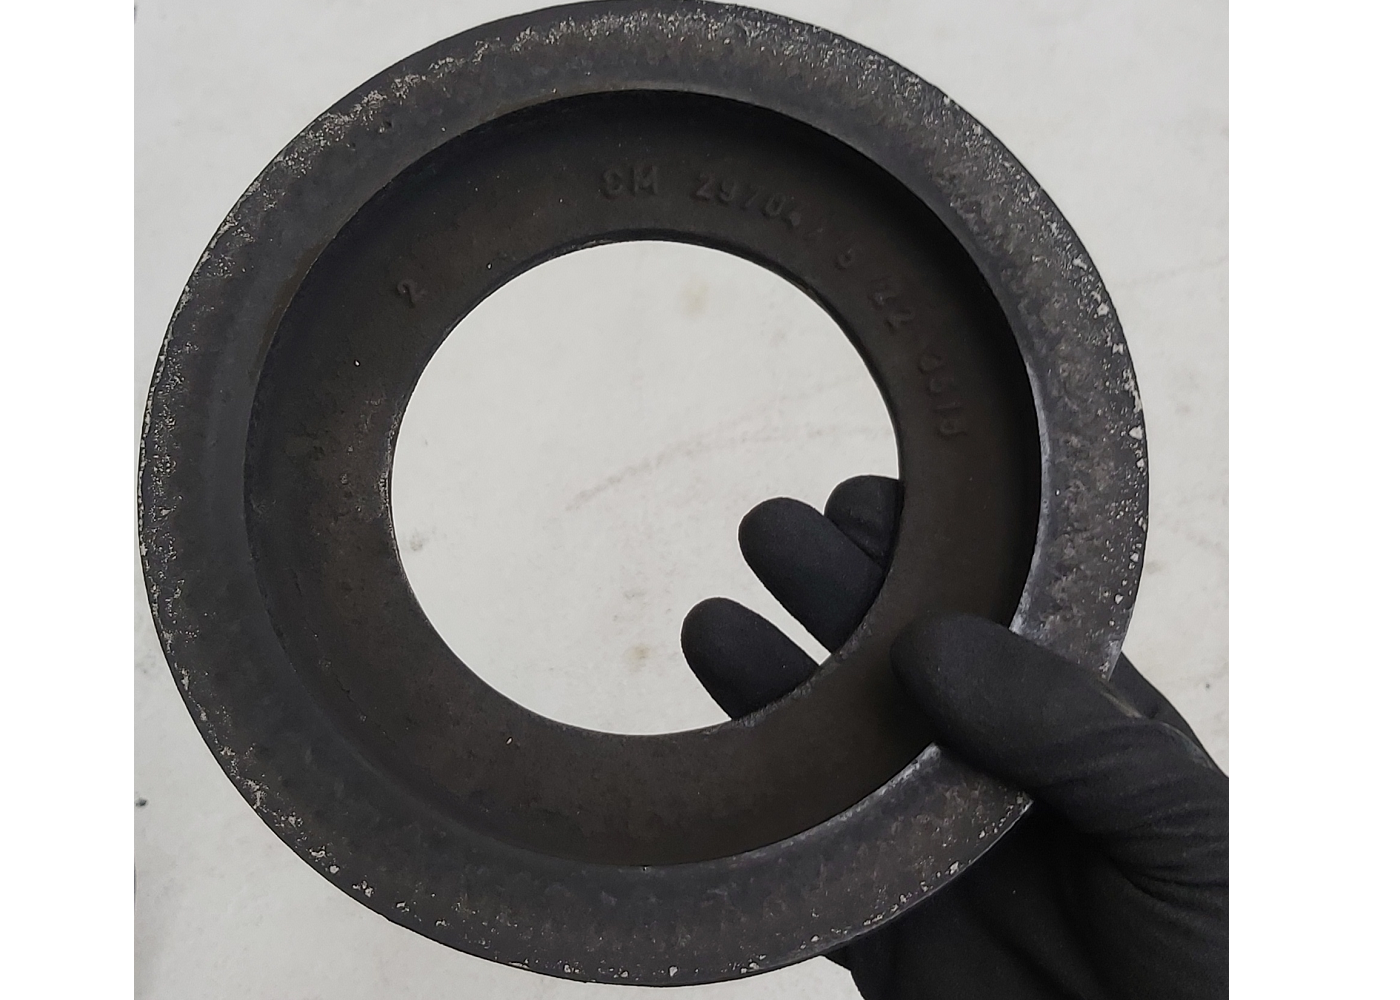
\includegraphics[width = 0.9\textwidth]{Figures/Cap3/Falsa_coroa.png}
        \caption{}
        \label{fig:Falsa_coroa}
    \end{subfigure}
    \caption[Fotografias dos tres componentes da ferramenta porta-peças]%
    {Fotografias do prato, da torre, e da falsa coroa da ferramenta porta-peças.}
\end{figure}
%%%%%%%%%%%%%%%%%%%%%%%%%%%%%%%%%%%%%%%%%%%%%%%%%%%%%%%%%%%%%%%%%%%%%%%%%%%%%
\par
A pré-oxidação é realizada ao aquecer o material a uma temperatura de 500\textdegree C por cerca de 90 minutos, num ambiente controlado, de forma a obter uma fina camada de óxidos na superfície das rodas de coroa que atua permitindo uma difusão mais controlada do carbono e do azoto na superfície do material durante a etapa de carbonitruração que resulta em uma distribuição mais uniforme destes elementos na camada formada, uniformizando as propriedades mecânicas adquiridas pelo processo. Para além disso, a camada de óxidos diminui a probabilidade de fissurações a quente, uma vez que funciona como um degrau de aquecimento e evita o choque térmico, já que o forno de carbonitruração encontra-se a temperaturas de quase 900\textdegree C. Por fim, a camada de óxidos também promove uma aderência mais forte entre a camada de carbonitruração e o núcleo metálico, o que diminui a probabilidade de ocorrência de descamações. Após esta etapa, as peças têm uma coloração característica, próxima do azul escuro, característica do processo de oxidação e da temperatura atingida neste processo.
\par
Logo após a pré-oxidação, as peças são conduzidas por transportadores mecânicos para um sitio de carregamento, para serem transportadas para o forno de carbonitruração. Neste forno, as peças são novamente aquecidas, desta vez a uma temperatura de 870\textdegree C, por um tempo de cerca de aproximadamente 180 minutos. Nesta etapa, as peças estão submetidas a uma atmosfera de aproximadamente 0,7\% Carbono e 20\% de Azoto, controladas por meio de um débito de amoníaco (NH\textsubscript{3}), metanol (CH\textsubscript{3}OH), propano (C\textsubscript{3}H\textsubscript{8}) e gás de azoto (N\textsubscript{2}). O processo é realizado numa câmara a uma pressão de 3 bar, de forma a permitir que a maior quantidade de átomos de carbono e azoto penetrem nas rodas de coroa.
%%%%%%%%%%%%%%%%%%%%%%%%%%%%%%%%%%%%%%%%%%%%%%%%%%%%%%%%%%%%%%%%%%%%%%%%%%%%%
\par
Após os aproximadamente 180 minutos no forno de carbonitruração, as peças são descarregadas do forno e rapidamente submergidas num tanque de têmpera de dimensões de base 700x700mm e  970mm de altura, num fluido de têmpera “Shell Voluta H300”, que encontra-se a aproximadamente 170\textdegree C durante cerca de 15 minutos. Após o processo de têmpera, as peças seguem para duas operações seguidas de lavagem, cada uma com duração de cerca de 90 minutos, e só então são submetidas à um processo de revenido, de forma a aliviar as tensões internas do material e adequar os valores de dureza e tenacidade às conformidade exigidas no produto final.
%%%%%%%%%%%%%%%%%%%%%%%%%%%%%%%%%%%%%%%%%%%%%%%%%%%%%%%%%%%%%%%%%%%%%%%%%%%%%
\begin{figure}[htb]
    \centering
    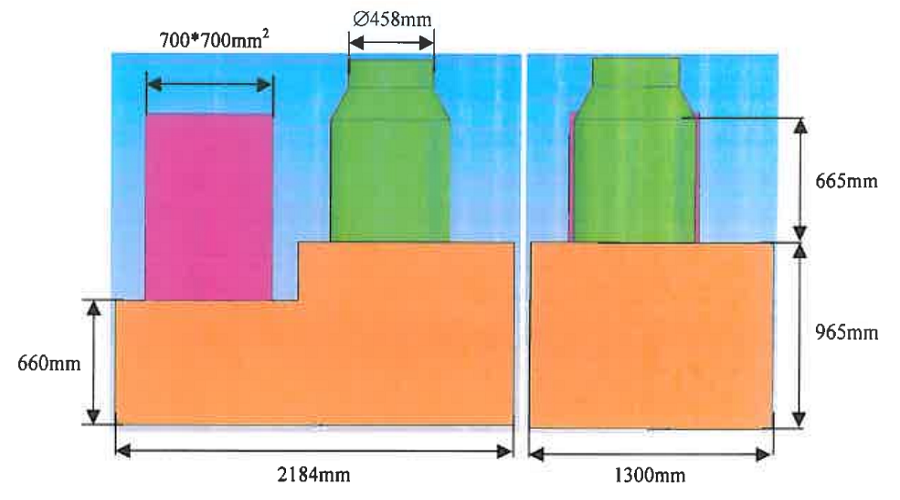
\includegraphics[width = 0.6\textwidth]{Figures/Cap3/Tanque_Tempera.png}
    \caption[Tanque de têmpera]%
    {Imagem esquemática do tanque de têmpera no qual é realizada a têmpera das rodas de coroa.}
    \label{fig:tanque_tempera}
\end{figure}
%%%%%%%%%%%%%%%%%%%%%%%%%%%%%%%%%%%%%%%%%%%%%%%%%%%%%%%%%%%%%%%%%%%%%%%%%%%%%

\par
O revenido é realizado durante 5 horas, em 5 zonas seguidas de 60 minutos cada, a 190\textdegree C, sendo então arrefecido lentamente à saída do forno de revenido. Após o arrefecimento das rodas de coroa, estas então são inseridas num processo de granalhagem, de forma limpar os contaminantes que restem dos processos anteriores, como resquícios de óleo não removidos no processo de lavagem, sobras de detergente ou camadas superficiais de óxidos. Uma vez que o processo de granalhagem é concluído, as rodas de coroa são conduzidas à linha de torneamento duro, onde serão removidas imperfeições e deformações resultantes do processo de obtenção da peça negra.

%%%%%%%%%%%%%%%%%%%%%%%%%%%%%%%%%%%%%%%%%%%%%%%%%%%%%%%%%%%%%%%%%%%%%%%%%%%%%
\newpage
\subsection{Processo de torneamento duro} \label{ssec:materiais_CS_torneamento}
Uma vez que as peças negras tem uma dureza superficial extremamente alta, por volta dos 700HV, é necessária a utilização de ferramentas e parâmetros de corte especiais para obter os requisitos dimensionais nas rodas de coroa. Para este efeito, são utilizadas pastilhas com revestimento de nitreto de boro cúbico (CBN), material este que pode atingir até 2000\textdegree C sem grandes perdas de dureza e em temperatura ambiente, apresenta valores de dureza por volta dos 1100HV. Neste processo, o diâmetro interno das rodas de coroa é torneada a zona de soldadura, a zona de prensagem, e é feito um rasgo para a zona de escapamento de gases de soldadura. As dimensões das rodas de coroa antes e depois do torneamento duro podem ser vistas nas Figuras \ref{fig:Coroa_antes_torneamento} e \ref{fig:Coroa_apos_torneamento}.
%%%%%%%%%%%%%%%%%%%%%%%%%%%%%%%%%%%%%%%%%%%%%%%%%%%%%%%%%%%%%%%%%%%%%%%%%%%%%
\begin{figure}[htb]
    \centering
    \begin{subfigure}{.5\textwidth}\
        \centering
        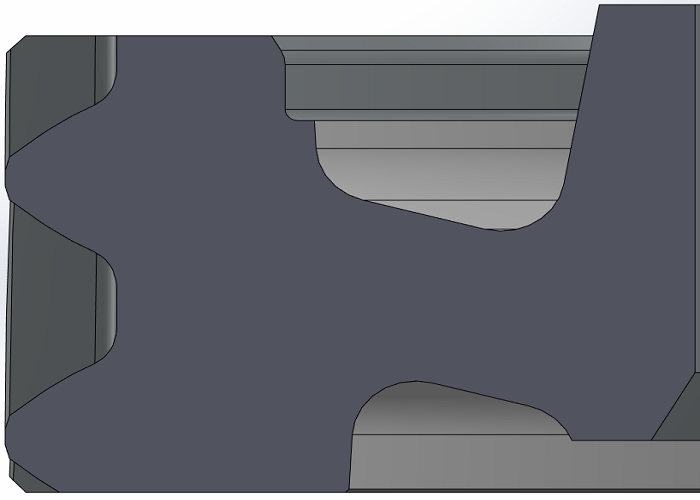
\includegraphics[width = 0.9\textwidth]{Figures/Cap3/DB45_antes_torn.png}
        \caption{}
        \label{fig:Coroa_antes_torneamento}
    \end{subfigure}%
    \begin{subfigure}{.5\textwidth}
        \centering
        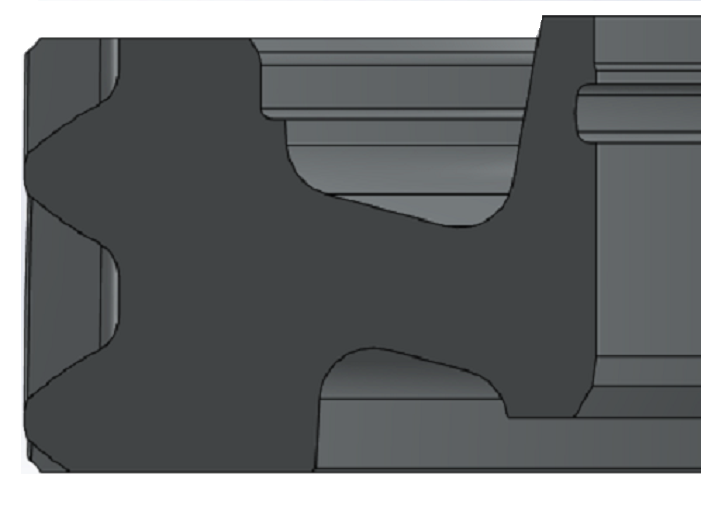
\includegraphics[width = 0.9\textwidth]{Figures/Cap3/DB45_apos_torn.png}
        \caption{}
        \label{fig:Coroa_apos_torneamento}
    \end{subfigure}
    \caption[Imagens das rodas de coroa antes e após o torneamento duro]%
    {À esquerda, um esquema das dimensões das rodas de coroa DB45 antes do torneamento duro. À direita, o mesmo esquema após a operação de torneamento duro, em vermelho, a zona de torneamento.}
\end{figure}
%%%%%%%%%%%%%%%%%%%%%%%%%%%%%%%%%%%%%%%%%%%%%%%%%%%%%%%%%%%%%%%%%%%%%%%%%%%%%

\par
Um dos problemas abordados neste projeto é justamente o custo da operação de torneamento duro. Os custos da ferramenta e a baixa quantidade de operações realizadas por cada ferramenta que resultam num tempo considerável em que a máquina não está a trabalhar e o alto consumo energético devido às condições de corte, que são maioritariamente causados pela alta dureza no diâmetro interno das rodas de coroa. 
%%%%%%%%%%%%%%%%%%%%%%%%%%%%%%%%%%%%%%%%%%%%%%%%%%%%%%%%%%%%%%%%%%%%%%%%%%%%%
\par
Sendo assim, havendo a possibilidade da redução desta dureza, existe uma margem para a diminuição dos custos de operação, seja com a mudança da ferramenta para uma alternativa de menor custo, pelo aumento da quantidade de operações realizadas por cada ferramenta, pela alteração dos parâmetros de corte de forma a reduzir o consumo energético ou o tempo de ciclo, ou até por uma junção de todas as possibilidades anteriores.
%%%%%%%%%%%%%%%%%%%%%%%%%%%%%%%%%%%%%%%%%%%%%%%%%%%%%%%%%%%%%%%%%%%%%%%%%%%%%
\subsection{Prensagem e Soldadura} \label{ssec:materials_CS_prens_e_sold}
Após o torneamento duro, as rodas de coroa são prensadas para em sequencia serem soldadas às caixas diferenciais, estas “caixas nuas”, em ferro fundido EN-GJS-600-10 são também produzidas na fábrica, no entanto, não sendo estas escopo deste projeto, seu processo produtivo não será abordado neste documento. Cada série de roda de coroa tem uma série de caixa diferencial designada, como exemplo, vê-se uma caixa diferencial “nua” na Figura \ref{fig:Caixa_nua_DB45}, e uma caixa diferencial montada na Figura \ref{fig:Caixa_montada_DB45}.
\newpage
%%%%%%%%%%%%%%%%%%%%%%%%%%%%%%%%%%%%%%%%%%%%%%%%%%%%%%%%%%%%%%%%%%%%%%%%%%%%%
\begin{figure}[htb]
    \centering
    \begin{subfigure}{.5\textwidth}\
        \centering
        \includegraphics[width = 0.9\textwidth]{Figures/Cap3/Caixa_nua.png}
        \caption[]%
        {}
        \label{fig:Caixa_nua_DB45}
    \end{subfigure}%
    \begin{subfigure}{.5\textwidth}
        \centering
        \includegraphics[width = 0.9\textwidth]{Figures/Cap3/Caixa_montada.png}
        \caption{}
        \label{fig:Caixa_montada_DB45}
    \end{subfigure}
    \caption[Caixa diferencial “nua”, e caixa diferencial montada.]%
    {À esquerda, uma fotografia de uma caixa diferencial “nua” antes de ser prensada a uma roda de coroa. À direita, uma caixa diferencial já prensada.}
\end{figure}
%%%%%%%%%%%%%%%%%%%%%%%%%%%%%%%%%%%%%%%%%%%%%%%%%%%%%%%%%%%%%%%%%%%%%%%%%%%%%
\par
Portanto, sendo prensadas a roda de coroa e caixa diferencial “nua”, a caixa diferencial deverá ser soldada, neste caso uma soldadura à laser com adição de INCONEL-82. Como referido no Subcapítulo \ref{ssec:soldadura-soldabilidade}, pode-se utilizar a correlação de Graville da Figura \ref{fig:Graville} para tentar prever a probabilidade de ocorrência de fissuração por hidrogénio no conjunto. Novamente, é importante referir que fissurações a hidrogénio são causadas por 3 fatores; microestrutura suscetível, neste caso, uma grande quantidade de martensite; uma fonte de hidrogénio difusível, neste caso, a atmosfera rica em hidrogénio da carbonitruração; e tensões residuais do processo de soldadura. Na Figura \ref{fig:microestrutura_diametro_serie} é possível verificar que o diâmetro interno das rodas de coroa estão preenchidas por microestruturas de martensite e austenite residual, com maior quantidade de austenite residual na extremidade mais próxima da superfície de tratamento. Isto pode ser explicado pela temperatura final de martensite de um aço ser mais baixa quanto maior a composição de carbono, e sendo a presença de carbono tão maior quanto menor for a profundidade observada, há uma maior presença de carbono na superfície, portanto, uma maior quantidade de austenite que não foi transformada.
%%%%%%%%%%%%%%%%%%%%%%%%%%%%%%%%%%%%%%%%%%%%%%%%%%%%%%%%%%%%%%%%%%%%%%%%%%%%%
\begin{figure}[htb]
    \centering
    \begin{subfigure}{.5\textwidth}\
        \centering
        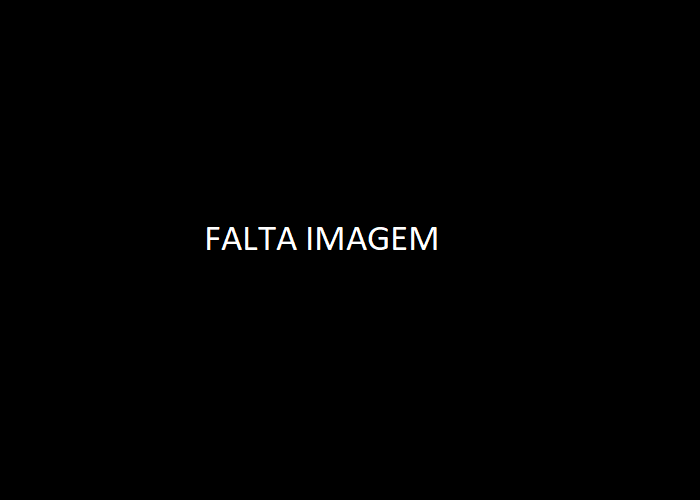
\includegraphics[width = 0.9\textwidth]{Figures/Cap3/Falta_Imagem.png}
        \caption{}
        \label{fig:microestrutura_diametro_serie}
    \end{subfigure}%
    \begin{subfigure}{.5\textwidth}
        \centering
        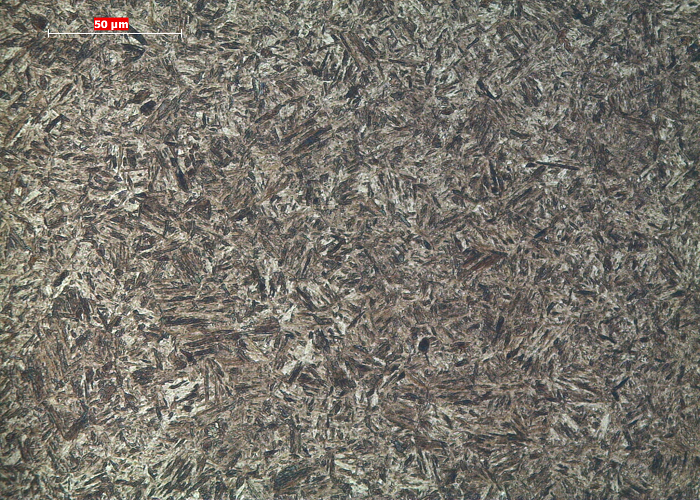
\includegraphics[width = 0.9\textwidth]{Figures/Cap3/Microestrutura_serie.png}
        \caption{}
        \label{fig:imagem_diametro_serie}
    \end{subfigure}
    \caption[Microestrutura e perfil do diâmetro interno.]%
    {À esquerda, uma imagem da microestrutura da peça branca. À direita, uma imagem da microestrutura de uma roda de coroa DB45 após têmpera.}
\end{figure}
%%%%%%%%%%%%%%%%%%%%%%%%%%%%%%%%%%%%%%%%%%%%%%%%%%%%%%%%%%%%%%%%%%%%%%%%%%%%%
%%%%%%%%%%%%%%%%%%%%%%%%%%%%%%%%%%%%%%%%%%%%%%%%%%%%%%%%%%%%%%%%%%%%%%%%%%%%%
\newpage
\par
Uma vez que os parâmetros de \% C e CE dos materiais da roda de coroa e da caixa “nua”, são importantes para perceber a suscetibilidade de fissuração por hidrogénio, a Tabela \ref{tab:Comp_materiais} indica a composição indicativa do aço 27MC5, das rodas de coroa, e do ferro fundido EN-GJS-600-10 das caixas diferenciais “nuas”. É importante referir que para o calculo posterior do CE, nas Equações \ref{eq:CE_calculado_27MC5} e \ref{eq:CE_calculado_GJS-600-10}, são utilizados os valores médios de cada elemento da composição do material, o que pode causar alguma diferença em materiais cuja composição se encontre numa posição mais extrema do espectro de conformidades. No entanto, uma vez que este espectro não é demasiado vasto, pode-se utilizar a média como visualização da soldabilidade deste material. Para além disso, é também utilizado o percentual de carbono após a carbonitruração, de 0,7\% , uma vez que a zona afetada termicamente das rodas de coroa de série é enriquecida por carbonitruração.
%%%%%%%%%%%%%%%%%%%%%%%%%%%%%%%%%%%%%%%%%%%%%%%%%%%%%%%%%%%%%%%%%%%%%%%%%%%%%
\begin{table}[htb]
    \centering
    \caption[Composição dos materiais da caixa diferencial]%
    {Valores de conformidade da composição dos materiais constituintes das rodas de coroa e caixas “nuas”.}
    \label{tab:Comp_materiais}
    \begin{tabular}{lrr} 
    \toprule
    \textbf{Elemento de liga} & \multicolumn{1}{c}{\textbf{Composição 27MC5 (\%)}} & \multicolumn{1}{c}{\textbf{Composição GJS-600-10 (\%)}}  \\ 
    \hline\hline
    Carbono (C)      & 0,23 à 0,31                               & 3,1 à 3,4                                       \\
    Manganês (Mn)    & 1,10 à 1,40                               & Até 0,5                                         \\
    Níquel (Ni)      & Até 0,30                                  & Não especificado                                \\
    Vanádio (V)      & Não especificado                          & Não especificado                                \\
    Molibdénio (Mo)  & Não especificado                          & Não especificado                                \\
    Crómio (Cr)      & 1,00 à 1,40                               & Não especificado                                \\
    Cobre (Cu)       & Até 0,40                                  & Até 0,15                                        \\
    Titânio (Ti)     & Até 0,010                                 & Não especificado                                \\
    Alumínio (Al)    & Até 0,050                                 & Não especificado                                \\
    Silício (Si)     & Até 0,40                                  & 4,1 à 4,5                                       \\
    Enxofre (S)      & 0,020 à 0,040                             & Até 0,02                                        \\
    Fósforo (P)      & Até 0,025                                 & Até 0,05                                        \\
    Estanho (Sn)     & Não especificado                          & Até 0,05                                        \\
    \bottomrule
    \end{tabular}
    \end{table}
%%%%%%%%%%%%%%%%%%%%%%%%%%%%%%%%%%%%%%%%%%%%%%%%%%%%%%%%%%%%%%%%%%%%%%%%%%%%%
%%%%%%%%%%%%%%%%%%%%%%%%%%%%%%%%%%%%%%%%%%%%%%%%%%%%%%%%%%%%%%%%%%%%%%%%%%%%%
\begin{equation}
    \centering
    \label{eq:CE_calculado_27MC5}
    \mathrm{CE\textsubscript{(27MC5)}} = 0,7 + \frac{1,25}{6}+\frac{1,20+0+0}{5}+\frac{0,20+0,15}{15}
\end{equation}
%%%%%%%%%%%%%%%%%%%%%%%%%%%%%%%%%%%%%%%%%%%%%%%%%%%%%%%%%%%%%%%%%%%%%%%%%%%%%
%%%%%%%%%%%%%%%%%%%%%%%%%%%%%%%%%%%%%%%%%%%%%%%%%%%%%%%%%%%%%%%%%%%%%%%%%%%%%
\begin{equation}
    \centering
    \label{eq:CE_calculado_GJS-600-10}
    \mathrm{CE\textsubscript{(GJS-600-10)}} = 3,25 + \frac{0,25}{6}+\frac{0+0+0}{5}+\frac{0,08+0}{15}
\end{equation}
%%%%%%%%%%%%%%%%%%%%%%%%%%%%%%%%%%%%%%%%%%%%%%%%%%%%%%%%%%%%%%%%%%%%%%%%%%%%%
\par
Com isto, temos que os valores de \%C e CE são, respetivamente 0,7 e 1,17 para o aço, e 3,25 e 3,3 para o ferro fundido. Quando comparados com os valores de referencia descritos na Tabela \ref{tab:CE}, ambos os materiais tem uma má soldabilidade, somado a isto, a martensite tem uma má condutividade térmica quando comparada com outras microestruturas do aço. 
\par
Ainda que usemos o valor de referencia para o percentual de carbono do aço sem tratamento termoquímico, temos um valor de CE de 0,72, o que ainda seria considerado um material com má soldabilidade. Devido a estes problemas, os parâmetros de soldadura são minuciosamente selecionados de forma a permitir uma boa formação da ZAT e uma penetração total da zona de soldadura, sendo o principal parâmetro para a obtenção destes resultados numa soldadura a laser a potencia de soldadura.
\newpage
\par
Para além disso, se utilizarmos a correlação de Graville, da Figura \ref{fig:Graville}, ambos os materiais têm uma grande probabilidade de ocorrência de fissuração, e o facto de serem peças de revolução, torna estas peças especialmente suscetíveis à fissurações, devido a zona de recobrimento (Figura \ref{fig:recobrimento}). Uma vez que a zona de inicio e término de soldadura da-se no mesmo ponto, esta zona sofre o equivalente a uma soldadura de dois passes. 
%%%%%%%%%%%%%%%%%%%%%%%%%%%%%%%%%%%%%%%%%%%%%%%%%%%%%%%%%%%%%%%%%%%%%%%%%%%%%
\begin{figure}[htb]
    \centering
    \includegraphics[width = 0.52\textwidth]{Figures/Cap3/Recobrimento.png}
    \caption[Zona de recobrimento de uma roda de coroa DB45]%
    {Fotografia de uma roda de coroa DB45 após o processo de soldadura, com destaque em vermelho para a zona de recobrimento.}
    \label{fig:recobrimento}
\end{figure}
%%%%%%%%%%%%%%%%%%%%%%%%%%%%%%%%%%%%%%%%%%%%%%%%%%%%%%%%%%%%%%%%%%%%%%%%%%%%%
\par
A adição de carbono, azoto, e a eventual adição de hidrogénio no forno de carbonitruração, e a transformação da microestrutura para martensite só aumentam a probabilidade de ocorrência de fissuração num conjunto que ja é extremamente suscetível a este fenómeno, portanto, uma vez que seja possível evitar o tratamento da zona de soldadura, seria possível diminuir a quantidade de não conformidades devidas aos defeitos de soldadura. Como ponto de comparação, a quantidade de peças não conformes devido aos defeitos de soldadura, ronda por volta das 1000 ppm, quantidade esta que aumenta demasiado o custo de fabrico das caixas diferenciais, uma vez que quaisquer não conformidades provenientes da soldadura resultam no sucateamento total da caixa, mesmo depois do processo produtivo estar quase completo.
%%%%%%%%%%%%%%%%%%%%%%%%%%%%%%%%%%%%%%%%%%%%%%%%%%%%%%%%%%%%%%%%%%%%%%%%%%%%%
\section{Conceção da ferramenta} \label{sec:materiais_concecao}
Tendo em conta os problemas descritos na secção anterior, cria-se a necessidade da conceção de uma ferramenta que impeça ou limite a existência dos efeitos que aumentam a probabilidade de ocorrência de fissurações à hidrogénio. Como a complexidade de tornar o diâmetro interno das rodas de coroa impermeáveis quanto à carbonitruração parece uma tarefa muito complicada, a primeira alternativa é tentar evitar a têmpera na zona do diâmetro interno.
%%%%%%%%%%%%%%%%%%%%%%%%%%%%%%%%%%%%%%%%%%%%%%%%%%%%%%%%%%%%%%%%%%%%%%%%%%%%%
\subsection{Simulação das peças de série} \label{ssec:materiais_concecao_sim_serie}
\par
De modo a perceber o comportamento das peças de série no tanque de têmpera, foi realizada uma simulação CFD do sistema. Para isto foi necessário modelar as três rodas de coroa de série (DB35, DB45 e JT4), bem como as ferramentas porta-peças atualmente utilizadas na etapa de carbonitruração.
\par
Estes modelos 3D foram realizados com o auxílio do software SolidWorks, e, de forma a evitar posteriormente quaisquer problemas quanto à construção da malha de elementos finitos e a simulação do sistema, optou-se por modelar as rodas de coroa sem os dentes, o que simplifica a construção da malha, sendo agora as rodas de coroa apenas um disco com um furo no centro, e diminui o número de elementos necessários para modelar o sistema. Os modelos das três rodas de coroa podem ser vistas nas Figuras \ref{fig:CAD_DB35}, \ref{fig:CAD_DB45} e \ref{fig:CAD_JT4}. Já para as ferramentas porta-peças, não foi necessário simplificar os modelos, uma vez que a geometria destes já é bastante simples e não traz grandes problemas em termos de construção de malha. O prato, a falsa coroa, e a torre podem ser vistos respetivamente nas Figuras \ref{fig:CAD_Prato}, \ref{fig:CAD_Falsa}, e \ref{fig:CAD_Torre}.
%%%%%%%%%%%%%%%%%%%%%%%%%%%%%%%%%%%%%%%%%%%%%%%%%%%%%%%%%%%%%%%%%%%%%%%%%%%%%
\begin{figure}[htb]
    \centering
    \begin{subfigure}{.33\textwidth}\
        \centering
        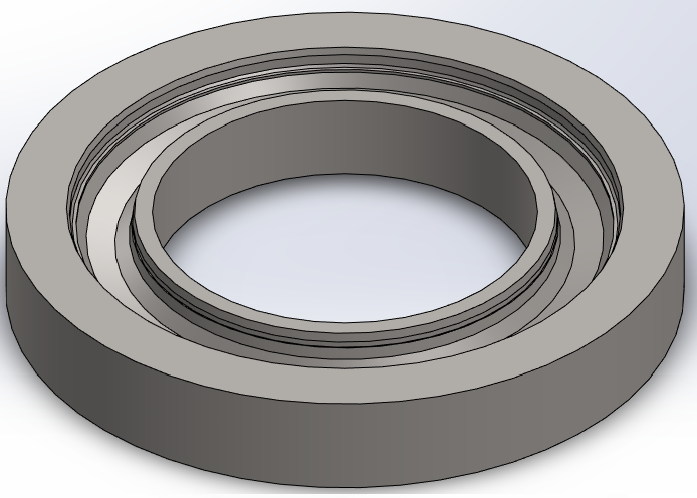
\includegraphics[width = 0.9\textwidth]{Figures/Cap3/CAD_DB35.png}
        \caption{}
        \label{fig:CAD_DB35}
    \end{subfigure}%
    \centering
    \begin{subfigure}{.33\textwidth}
        \centering
        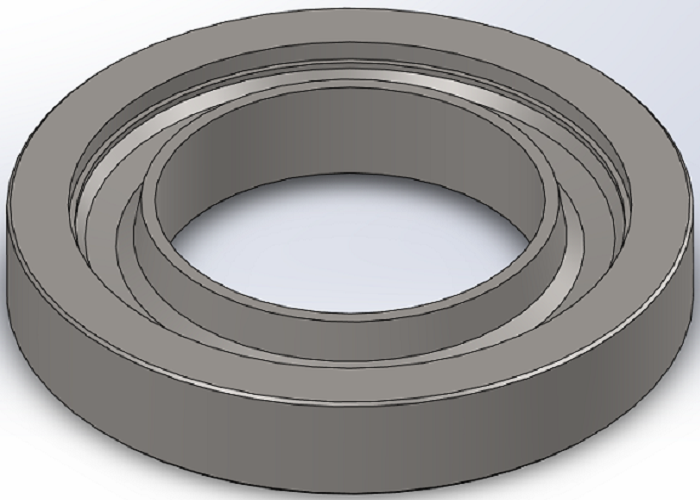
\includegraphics[width = 0.9\textwidth]{Figures/Cap3/CAD_DB45.png}
        \caption{}
        \label{fig:CAD_DB45}
    \end{subfigure}
    \centering
    \begin{subfigure}{.33\textwidth}
        \centering
        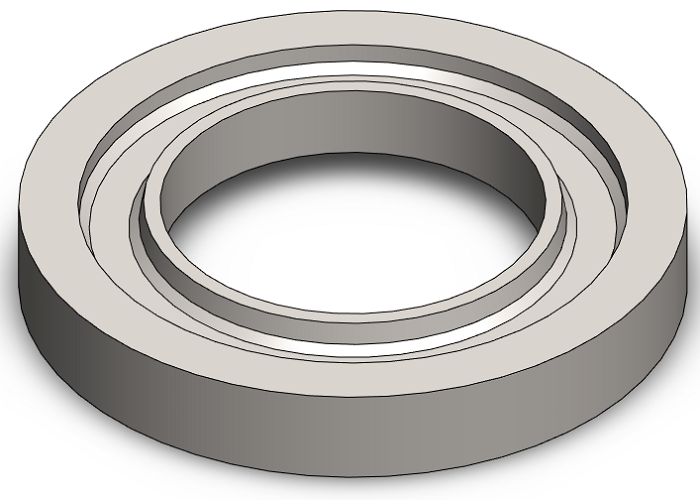
\includegraphics[width = 0.9\textwidth]{Figures/Cap3/CAD_JT4.png}
        \caption{}
        \label{fig:CAD_JT4}
    \end{subfigure}
    \centering
    \begin{subfigure}{.33\textwidth}\
        \centering
        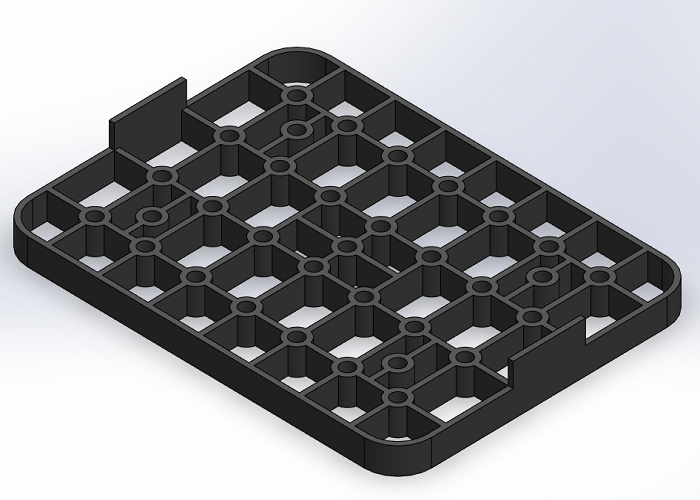
\includegraphics[width = 0.9\textwidth]{Figures/Cap3/CAD_PRATO.png}
        \caption{}
        \label{fig:CAD_Prato}
    \end{subfigure}%
    \centering
    \begin{subfigure}{.33\textwidth}
        \centering
        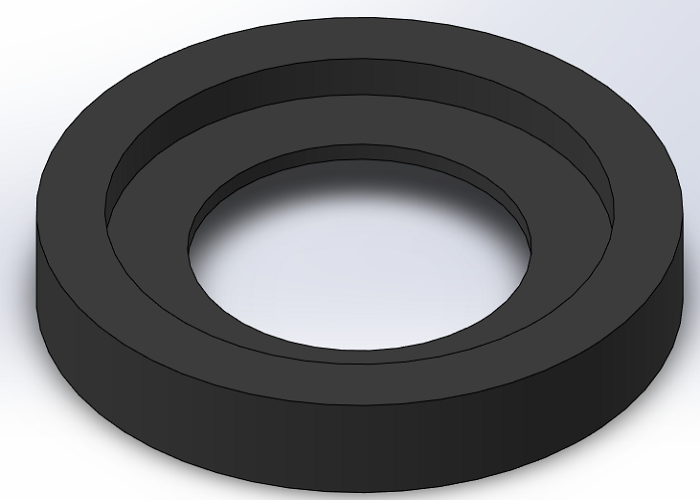
\includegraphics[width = 0.9\textwidth]{Figures/Cap3/CAD_FALSA.png}
        \caption{}
        \label{fig:CAD_Falsa}
    \end{subfigure}
    \centering
    \begin{subfigure}{.33\textwidth}
        \centering
        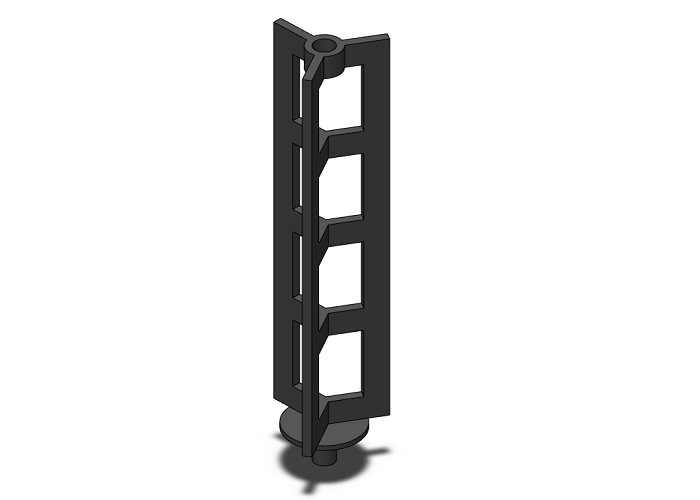
\includegraphics[width = 0.9\textwidth]{Figures/Cap3/CAD_TORRE.png}
        \caption{}
        \label{fig:CAD_Torre}
    \end{subfigure}
    \caption[Modelos 3D das rodas de coroa e dos elementos da ferramenta porta-peças.]%
    {\textbf{(a)} Modelo CAD 3D de uma roda de coroa DB35; \textbf{(b)} Modelo de uma roda de coroa DB45; \textbf{(c)} Modelo de uma roda de coroa JT4; \textbf{(d)} Modelo de um prato da ferramenta porta-peças; \textbf{(e)} Modelo de uma falsa coroa da ferramenta porta-peças; \textbf{(a)} Modelo de uma torre da ferramenta porta-peças.}
\end{figure}
%%%%%%%%%%%%%%%%%%%%%%%%%%%%%%%%%%%%%%%%%%%%%%%%%%%%%%%%%%%%%%%%%%%%%%%%%%%%%
% \par
% Após todos os elementos do sistema estarem modelados, realizou-se a montagem do sistema a ser simulado. Basicamente, como no porta-peças real, cada prato contêm 5 torres, e cada torre contem 10 rodas de coroa, no caso da DB45 e 11 rodas de coroa, no caso da DB35 e JT4.
%%%%%%%%%%%%%%%%%%%%%%%%%%%%%%%%%%%%%%%%%%%%%%%%%%%%%%%%%%%%%%%%%%%%%%%%%%%%%
\begin{table}[htb]
    \centering
    \caption[Propriedades mecânicas e térmicas do aço 27MC5]%
    {Propriedades mecânicas e térmicas do aço 27MC5 usadas nas simulações CFD.}
    \label{tab:Propriedades_27MC5}
    \begin{tabular}{lrr} 
    \toprule
    \multicolumn{1}{c}{\textbf{Propriedades}} & \multicolumn{1}{c}{\textbf{Aço 27MC5}}            & \multicolumn{1}{c}{\textbf{Refratário EN 1.4807}}  \\ 
    \hline\hline
    Densidade ($\rho$)                        & 7800 kg m\textsuperscript{-3}                     & 8000 kg m\textsuperscript{-3}                      \\
    Módulo de Young (E)                       & 190 GPa                                           & 190 GPa                                            \\
    Coeficiente de poisson ($\nu$)            & 0,29                                              & 0,29                                               \\
    Tensão de limite elástico (\textit{T})             & 380 MPa                                           & 120 MPa                                            \\
    Coef. de expansão térmica (\textit{a})             & 0,13 $\mu$K\textsuperscript{-1}                   & 0,15 $\mu$K\textsuperscript{-1}                    \\
    Coef. de condutividade térmica (\textit{K})        & 46 W m\textsuperscript{-1}K\textsuperscript{-1}   & 12 W m\textsuperscript{-1}K\textsuperscript{-1}    \\
    Calor específico (\textit{c})                      & 470 J kg\textsuperscript{-1}K\textsuperscript{-1} & 480 J kg\textsuperscript{-1}K\textsuperscript{-1}  \\
    \toprule
    \end{tabular}
    \end{table}
%%%%%%%%%%%%%%%%%%%%%%%%%%%%%%%%%%%%%%%%%%%%%%%%%%%%%%%%%%%%%%%%%%%%%%%%%%%%%
\newpage
\par
Uma vez que o modelo CFD necessita de alguns dados dos materiais e do fluido térmico, estes podem ser encontrados nas Tabelas \ref{tab:Propriedades_27MC5} e \ref{tab:Propriedades_VolutaH300}, e uma imagem do modelo montado pode ser vista na Figura \ref{fig:modelo_montado}
%%%%%%%%%%%%%%%%%%%%%%%%%%%%%%%%%%%%%%%%%%%%%%%%%%%%%%%%%%%%%%%%%%%%%%%%%%%%%
\begin{table}[htb]
    \centering
    \caption[Propriedades do fluido de têmpera Voluta H300]%
    {Propriedades mecânicas e térmicas do aço 27MC5 usadas nas simulações CFD.}
    \label{tab:Propriedades_VolutaH300}
    \begin{tabular}{lrrr} 
    \toprule
    \multicolumn{1}{c}{\textbf{Propriedades Voluta H300}} & \multicolumn{1}{c}{\textbf{20 °C}} & \multicolumn{1}{c}{\textbf{100 °C}} & \multicolumn{1}{c}{\textbf{140 °C}}  \\ 
    \hline\hline
    Densidade ($\rho$)                                    & 780 kg m\textsuperscript{-3}       & 600 kg m\textsuperscript{-3}        & 600 kg m\textsuperscript{-3}         \\
    Viscosidade cinemática ($\mu$)                        & 571 cSt                            & 190 cSt                             & 4,8 cSt                              \\
    Temperatura de transf. de fase (\textit{T})           & \multicolumn{3}{c}{400 °C}                                                                                      \\
    Coef. de condutividade térmica (\textit{K})           & \multicolumn{3}{c}{46 W m\textsuperscript{-1}K\textsuperscript{-1}}                                             \\
    Calor específico (\textit{cp})                        & \multicolumn{3}{c}{470 J kg\textsuperscript{-1}K\textsuperscript{-1}}                                           \\
    \bottomrule
    \end{tabular}
    \end{table}
%%%%%%%%%%%%%%%%%%%%%%%%%%%%%%%%%%%%%%%%%%%%%%%%%%%%%%%%%%%%%%%%%%%%%%%%%%%%%
%%%%%%%%%%%%%%%%%%%%%%%%%%%%%%%%%%%%%%%%%%%%%%%%%%%%%%%%%%%%%%%%%%%%%%%%%%%%%
\begin{figure}[htb]
    \centering
    \begin{subfigure}{.5\textwidth}\
        \centering
        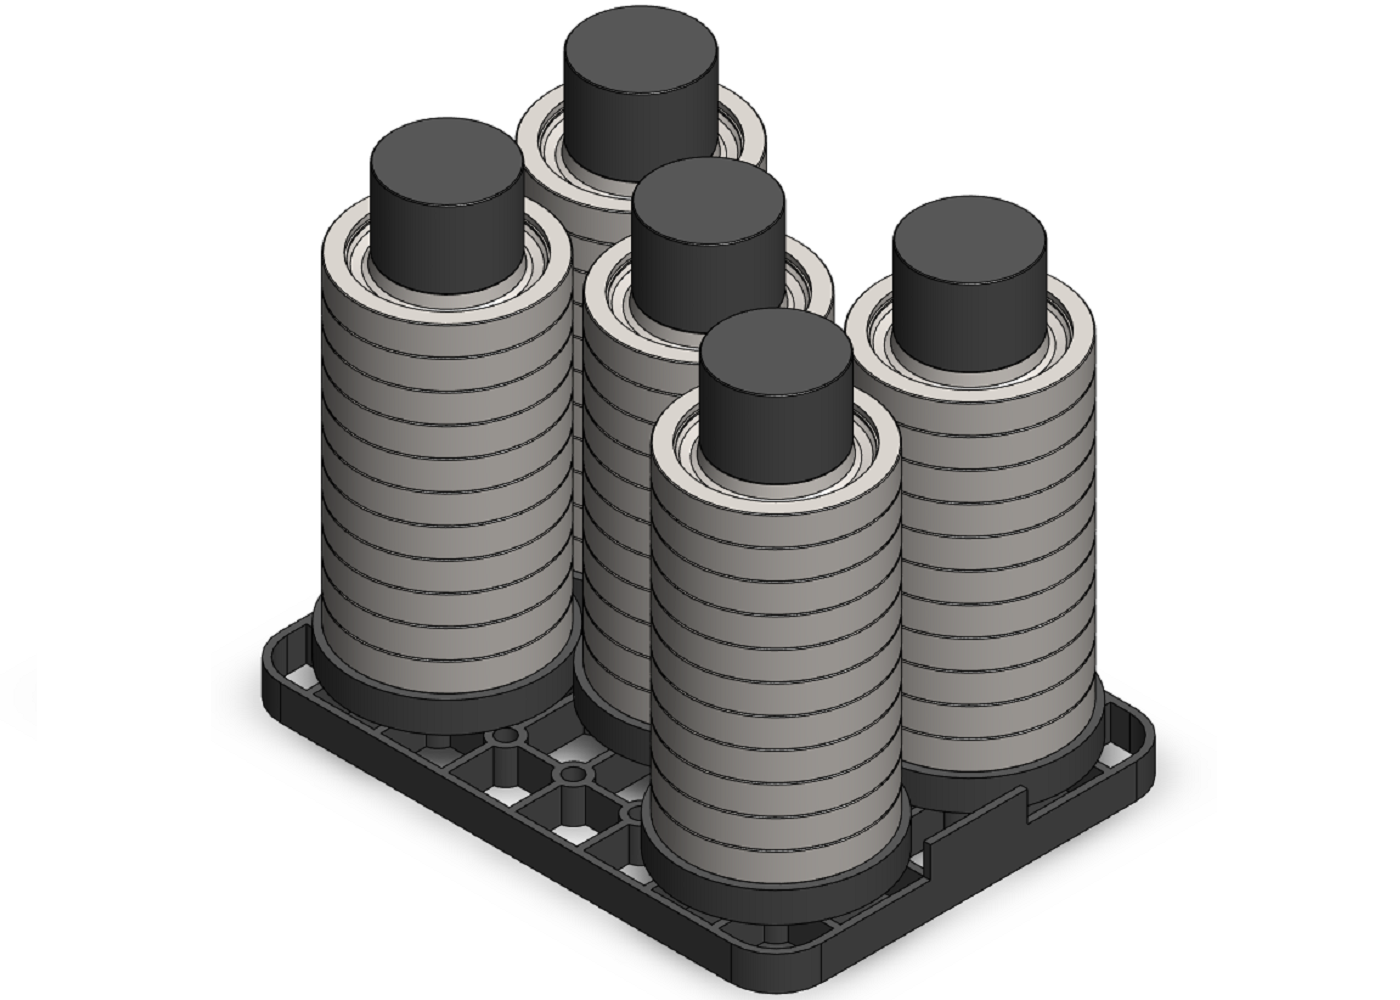
\includegraphics[width = 0.9\textwidth]{Figures/Cap3/Prato_montado.png}
        \caption{}
        \label{fig:modelo_montado}
    \end{subfigure}%
    \begin{subfigure}{.5\textwidth}
        \centering
        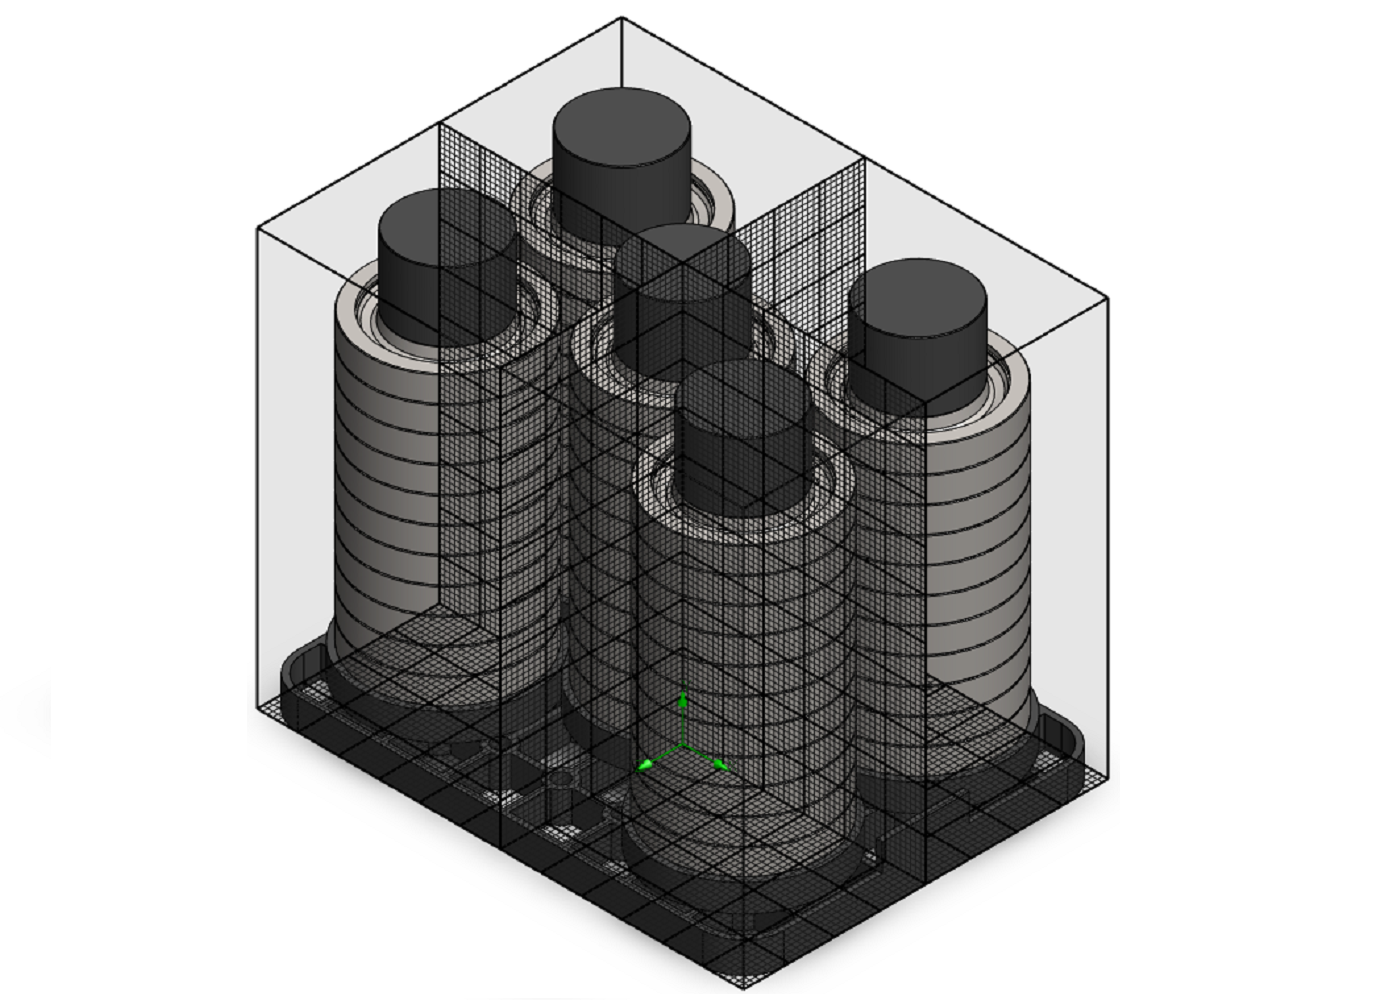
\includegraphics[width = 0.9\textwidth]{Figures/Cap3/Prato_montado_malha.png}
        \caption{}
        \label{fig:malha_simulacao}
    \end{subfigure}
    \caption[Modelo 3D de um prato montado e esquema de malhas da simulação.]%
    {À esquerda, modelo CAD 3D de um prato de rodas de coroa DB45 montado. À direita, esquema de malhas utilizado na simulação CFD.}
\end{figure}
%%%%%%%%%%%%%%%%%%%%%%%%%%%%%%%%%%%%%%%%%%%%%%%%%%%%%%%%%%%%%%%%%%%%%%%%%%%%%
\par
Por fim, utiliza-se o add-on \textit{Flow Simulation} do software SolidWorks para criar um programa de simulações, de forma a visualizar o comportamento do fluido de têmpera nas condições de tratamento. Para além dos dados indicados nas tabelas acima, às peças foi definida uma temperatura de 870 \textdegree C, e foram utilizados um coeficiente de rugosidade em todas as faces das rodas de coroa de 50$\mu$m, uma rugosidade de 500 $\mu$m em todas as faces dos componentes da ferramenta porta-peças, e foi definida uma malha “grosseira” para os elementos sólidos, e uma malha “normal” para os elementos de fluido. Ver Figura \ref{fig:malha_simulacao}.
\par
Os limites computacionais do fluido foram definidos de acordo com as dimensões do tanque que encontra-se descrito na Figura \ref{fig:tanque_tempera}, ou seja, (700x700) mm\textsuperscript{2} de base e 900 mm de altura, e o plano inferior do tanque foi assumido como uma entrada uniforme de fluido de tempera a uma velocidade de 1,45 m/s, e a uma temperatura de 170 \textdegree C de acordo com o documento do tanque que pode ser visualizado no Apêndice \ref{ap:tanque_tempera}.
\newpage
\par
Uma vez que, mesmo com geometrias pouco complexas e com a utilização de uma malha “grosseira” nos elementos sólidos, a simulação em questão tem um grande custo computacional, esta consumiu cerca de 9 horas até estar completa, e com isto, como pode ser visto na Figura \ref{fig:resultado_serie}, é possível  que o fluxo de fluido é tão grande ou talvez até mais volumoso no diâmetro interno das rodas de coroa que no dentado, portanto, confirmando mais uma vez que é realizada uma têmpera no diâmetro interno da mesma maneira que no dentado. No entanto, não há necessidade da existência de grandes durezas no diâmetro interno, e a presença de martensite é indesejada, por conta da ocorrência de fissurações a hidrogénio.
% \par
% Dito isso, confirma-se a necessidade da conceção de um sistema de tamponamento para evitar o fluxo de fluido térmico por este diâmetro, ao adicionar uma “tampa” simples, e soldar a coluna á falsa coroa, criando assim uma “geometria protegida” contra a têmpera.
%%%%%%%%%%%%%%%%%%%%%%%%%%%%%%%%%%%%%%%%%%%%%%%%%%%%%%%%%%%%%%%%%%%%%%%%%%%%%
\begin{figure}[htb]
    \centering
    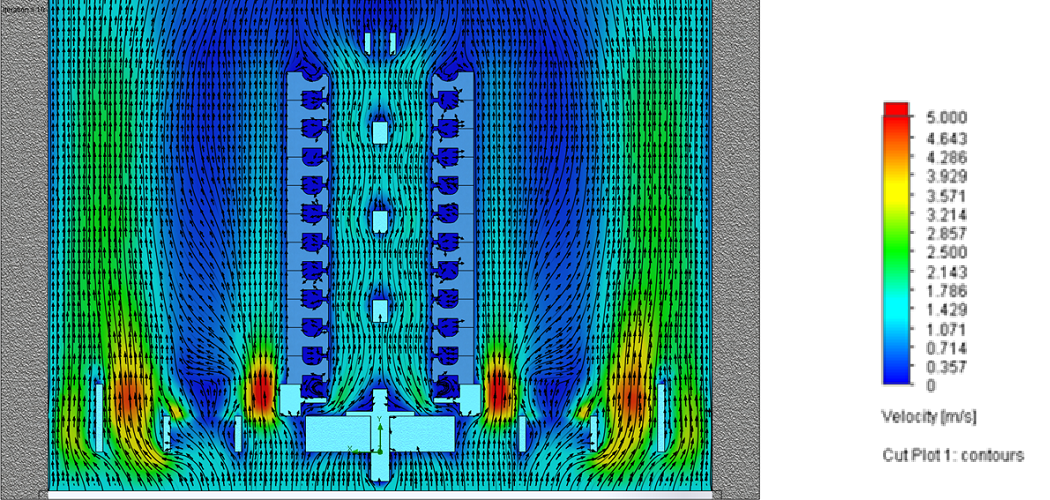
\includegraphics[width = 0.8\textwidth]{Figures/Cap3/resultado_serie.png}
    \caption[Resultado da simulação CFD da têmpera das rodas de coroa de série]%
    {Imagem de um corte no plano XZ, a meio da coluna central, do fluxo de fluido resultante da imersão do prato de rodas de coroa DB45 de série no tanque de têmpera, onde o gradiente de cores corresponde à velocidade do fluido, com \colorbox{Blue}{\textcolor{White}{azul escuro sendo 0 m/s}}, e \colorbox{Red}{\textcolor{White}{vermelho sendo 5 m/s ou maior.}}}
    \label{fig:resultado_serie}
\end{figure}
%%%%%%%%%%%%%%%%%%%%%%%%%%%%%%%%%%%%%%%%%%%%%%%%%%%%%%%%%%%%%%%%%%%%%%%%%%%%%
\subsection{Simulação da tampa simples}  \label{ssec:materiais_concecao_simples}
Como visto ser necessário na subsecção anterior, foi desenvolvida uma nova ferramenta porta-peças para proteger o diâmetro interno, com uma tampa na parte superior (Ver Figura \ref{fig:tampa_simples}), e onde se aproveitou a falsa coroa, a torre e o prato, foi adicionado um copo para permitir a soldadura da torre na falsa coroa (Ver \ref{fig:falsa_coroa_torre}). A imagem da ferramenta porta-peças e uma vista em corte, com uma coluna de rodas de coroa DB45 montada pode ser vista nas Figuras \ref{fig:simples_montada}, e \ref{fig:simples_corte}, respetivamente.

%%%%%%%%%%%%%%%%%%%%%%%%%%%%%%%%%%%%%%%%%%%%%%%%%%%%%%%%%%%%%%%%%%%%%%%%%%%%%
\begin{figure}[htb]
    \centering
    \begin{subfigure}{.5\textwidth}\
        \centering
        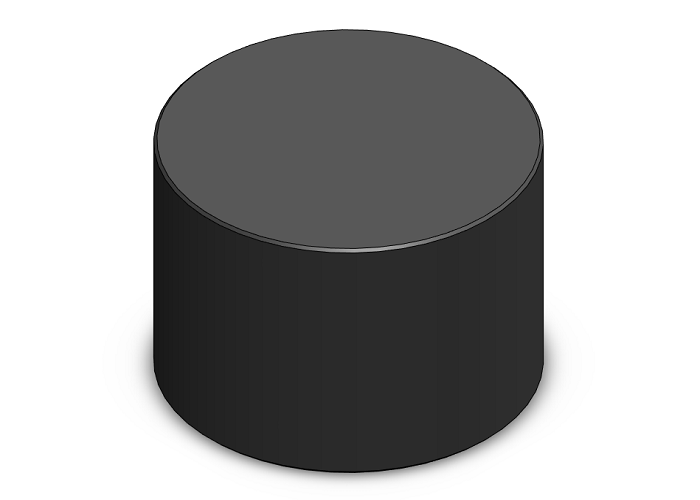
\includegraphics[width = 0.5\textwidth]{Figures/Cap3/Tampa_P.png}
        \caption{}
        \label{fig:tampa_simples}
    \end{subfigure}%
    \begin{subfigure}{.5\textwidth}
        \centering
        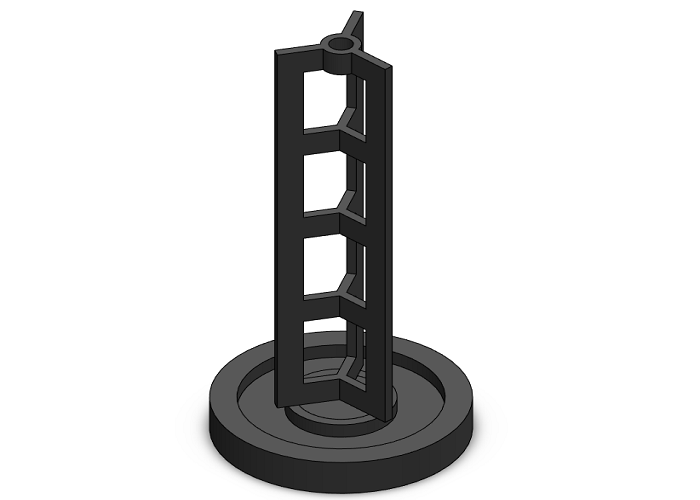
\includegraphics[width = 0.5\textwidth]{Figures/Cap3/Falsa_coroa_modificada.png}
        \caption{}
        \label{fig:falsa_coroa_torre}
    \end{subfigure}
    \caption[Imagens ilustrativas dos componentes modificados da proposta inicial.]%
    {Imagens ilustrativas em CAD 3D dos sistemas que compõem a proposta inicial da ferramenta porta-peças com diâmetro protegido.}
\end{figure}
%%%%%%%%%%%%%%%%%%%%%%%%%%%%%%%%%%%%%%%%%%%%%%%%%%%%%%%%%%%%%%%%%%%%%%%%%%%%%
\newpage
%%%%%%%%%%%%%%%%%%%%%%%%%%%%%%%%%%%%%%%%%%%%%%%%%%%%%%%%%%%%%%%%%%%%%%%%%%%%%
\begin{figure}[htb]
    \centering
    \begin{subfigure}{.5\textwidth}\
        \centering
        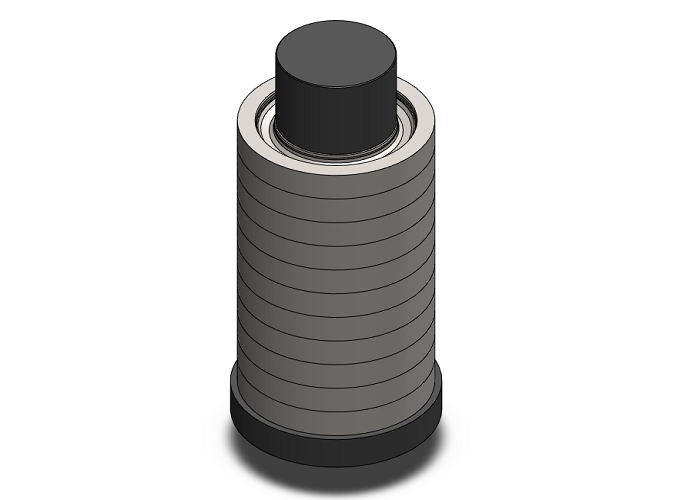
\includegraphics[width = 0.7\textwidth]{Figures/Cap3/Coluna_P_Montada.png}
        \caption{}
        \label{fig:simples_montada}
    \end{subfigure}%
    \begin{subfigure}{.5\textwidth}
        \centering
        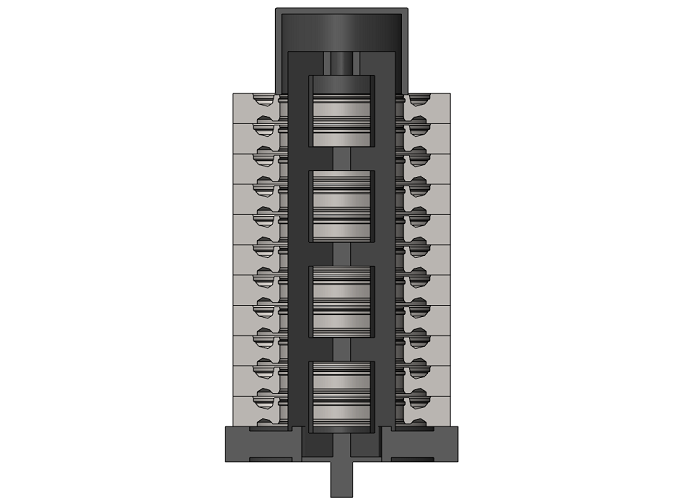
\includegraphics[width = 0.7\textwidth]{Figures/Cap3/Coluna_P_Montada_Corte.png}
        \caption{}
        \label{fig:simples_corte}
    \end{subfigure}
    \caption[Imagens ilustrativas da proposta inicial montada e em corte.]%
    {Imagens ilustrativas em CAD 3D do sistema montado com uma coluna de rodas de coroa DB45 em vista isométrica e em vista frontal em corte.}
\end{figure}
%%%%%%%%%%%%%%%%%%%%%%%%%%%%%%%%%%%%%%%%%%%%%%%%%%%%%%%%%%%%%%%%%%%%%%%%%%%%%
\par
Tendo o modelo CAD da ferramenta, fez-se então uma simulação nos mesmos parâmetros definidos para o sistema de série, podendo o resultado do fluxo de fluido térmico ser observado na Figura \ref{fig:resultado_simples}. Como é possível observar, o fluxo de fluido térmico é um pouco afetado no dentado das rodas de coroa inferiores, no entanto, não há quase nenhum fluxo de fluido térmico dentro da geometria que se deseja proteger, o que indica que provavelmente haverá pouca ou nenhuma têmpera nos diâmetros internos das rodas de coroa com este tipo de ferramenta porta-peças.
%%%%%%%%%%%%%%%%%%%%%%%%%%%%%%%%%%%%%%%%%%%%%%%%%%%%%%%%%%%%%%%%%%%%%%%%%%%%%
\begin{figure}[htb]
    \centering
    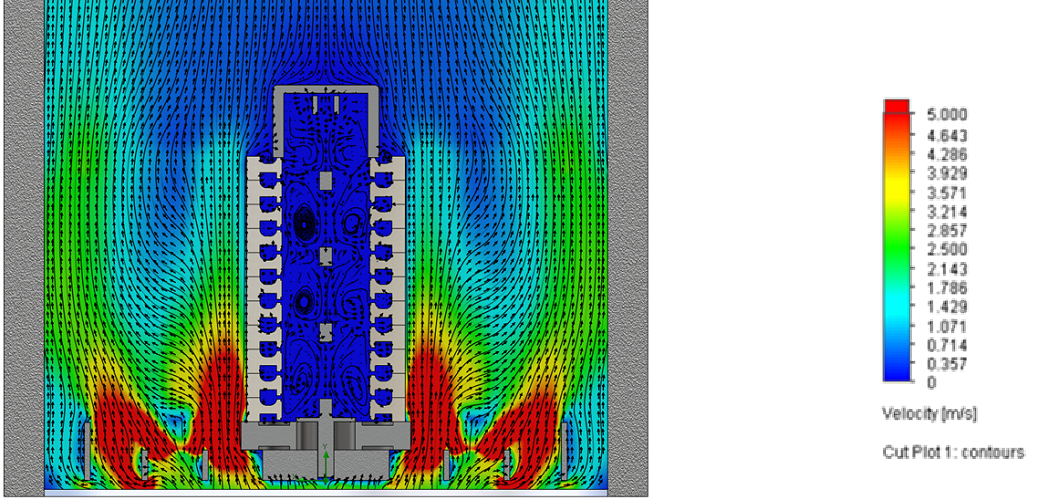
\includegraphics[width = 0.8\textwidth]{Figures/Cap3/resultado_simples.png}
    \caption[Resultado da simulação CFD da têmpera das rodas de coroa com diâmetro protegido]%
    {Imagem de um corte no plano XZ, a meio da coluna central, do fluxo de fluido resultante da imersão do prato de rodas de coroa DB45 com diâmetro protegido no tanque de têmpera, onde o gradiente de cores corresponde à velocidade do fluido, com \colorbox{Blue}{\textcolor{White}{azul escuro sendo 0 m/s}}, e \colorbox{Red}{\textcolor{White}{vermelho sendo 5 m/s ou maior.}}}
    \label{fig:resultado_simples}
\end{figure}
%%%%%%%%%%%%%%%%%%%%%%%%%%%%%%%%%%%%%%%%%%%%%%%%%%%%%%%%%%%%%%%%%%%%%%%%%%%%%
\newpage
\subsection{Prototipagem da tampa simples}  \label{ssec:materiais_prototipagem_simples}
Tendo então resultados satisfatórios na simulação, prosseguiu-se com a próxima etapa da conceção da ferramenta. Para verificar que as dimensões geométricas estavam compatíveis com os sistemas produtivos, fez-se uma impressão 3D dos componentes modificados que podem ser vistos nas Figuras \ref{fig:Tampa_simples_3d}, \ref{fig:falsa_coroa_torre_3d}. Estes componentes tiveram suas dimensões verificadas num prato de rodas de coroa de série DB45. Verificadas as dimensões, como pode ser visto na Figura \ref{fig:teste_impressao_3d}, prosseguiu-se com a ordem de trabalho para maquinar uma tampa simples e modificar a torre e a falsa coroa, de forma a realizar um ensaio de tratamento térmico, para verificar a microestrutura e as durezas e comparar os resultados com as rodas de coroa de série.
%%%%%%%%%%%%%%%%%%%%%%%%%%%%%%%%%%%%%%%%%%%%%%%%%%%%%%%%%%%%%%%%%%%%%%%%%%%%%
\begin{figure}[htb]
    \centering
    \begin{subfigure}{.5\textwidth}\
        \centering
        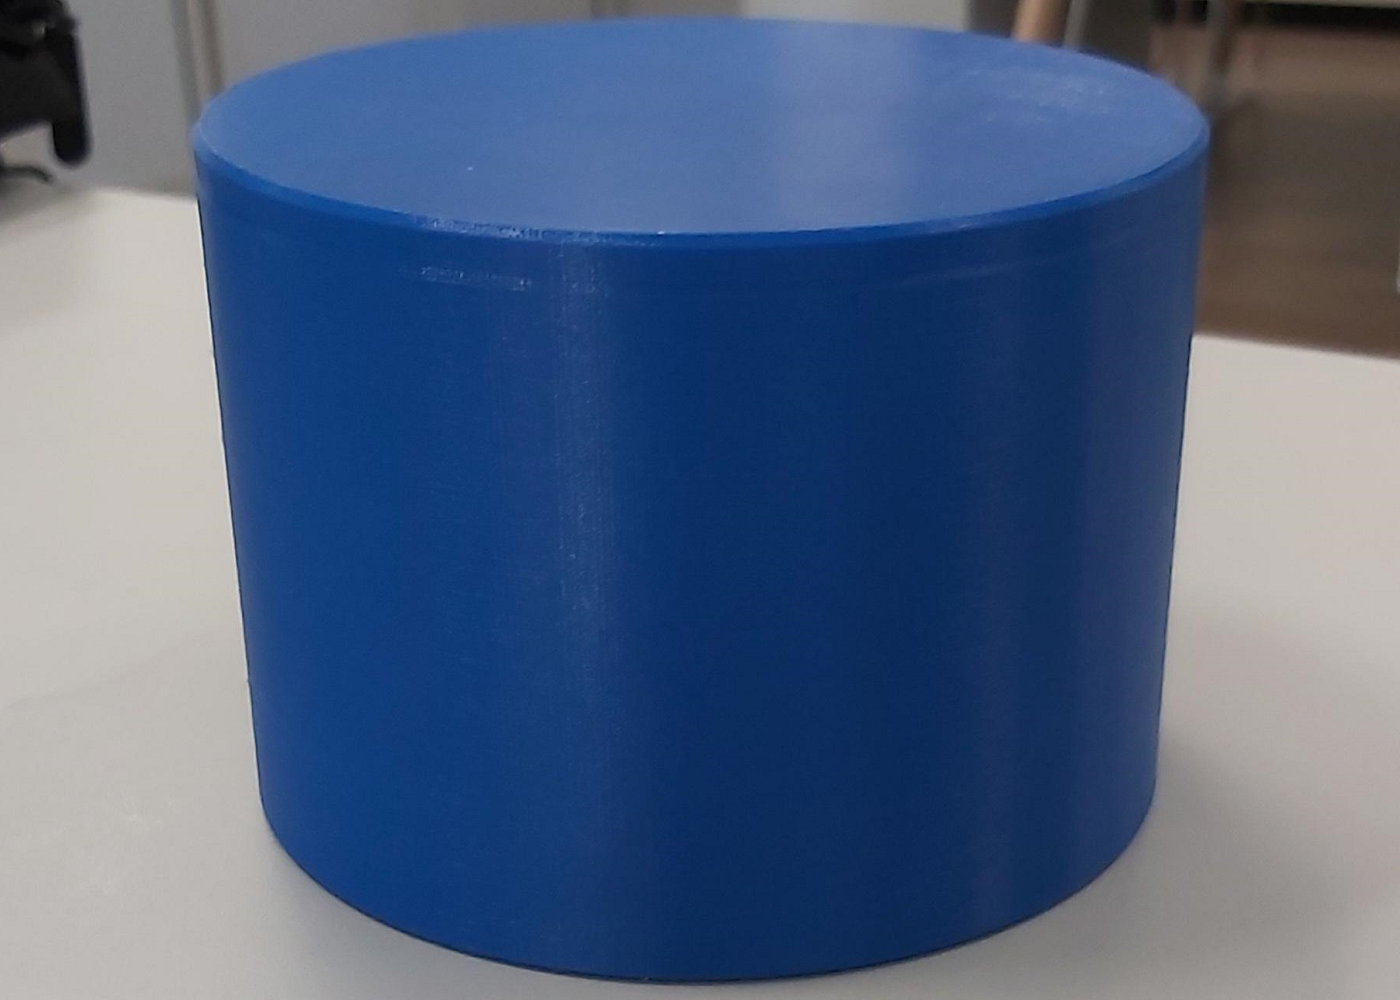
\includegraphics[width = 0.9\textwidth]{Figures/Cap3/tampa_simples_3d.png}
        \caption{}
        \label{fig:Tampa_simples_3d}
    \end{subfigure}%
    \begin{subfigure}{.5\textwidth}
        \centering
        \includegraphics[width = 0.9\textwidth]{Figures/Cap3/Falsa_coroa_torre_3d.png}
        \caption{}
        \label{fig:falsa_coroa_torre_3d}
    \end{subfigure}
    \caption[Modelos dos componentes modificados impressos em PET-G.]%
    {Modelos impressos em PET-G no laboratório de impressão 3D da Renault Cacia, Á direita a tampa simples e à esquerda, a falsa coroa soldada à torre. Toda a impressão foi feita durante o fim de semana e durou mais de 40 horas.}
\end{figure}
%%%%%%%%%%%%%%%%%%%%%%%%%%%%%%%%%%%%%%%%%%%%%%%%%%%%%%%%%%%%%%%%%%%%%%%%%%%%%
%%%%%%%%%%%%%%%%%%%%%%%%%%%%%%%%%%%%%%%%%%%%%%%%%%%%%%%%%%%%%%%%%%%%%%%%%%%%%
\begin{figure}[htb]
    \centering
    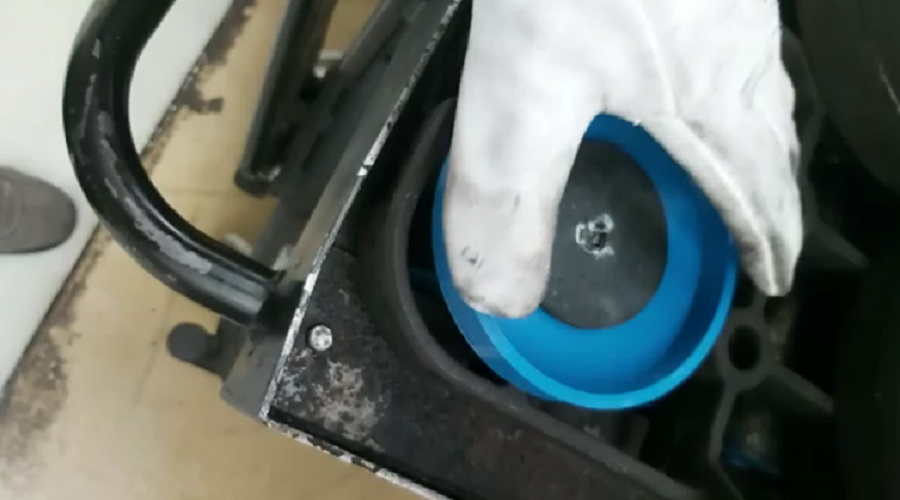
\includegraphics[width = 0.9\textwidth]{Figures/Cap3/Teste_impressao_largo.png}
    \caption[Teste dos componentes impressos em 3D no prato e nas rodas de coroa]%
    {Fotografia do teste dos componentes impressos em 3D no prato e nas rodas de coroa, para verificar se as dimensões projetadas são compatíveis com os componentes já existentes.}
    \label{fig:teste_impressao_3d}
\end{figure}
%%%%%%%%%%%%%%%%%%%%%%%%%%%%%%%%%%%%%%%%%%%%%%%%%%%%%%%%%%%%%%%%%%%%%%%%%%%%%
\newpage
%%%%%%%%%%%%%%%%%%%%%%%%%%%%%%%%%%%%%%%%%%%%%%%%%%%%%%%%%%%%%%%%%%%%%%%%%%%%%
\subsection{Ensaio da proposta inicial} \label{ssec:materiais_ensaio_simples}
Como referido na subsecção anterior, foi realizado um ensaio da ferramenta modificada, onde o objetivo era verificar se os resultados obtidos pela simulação CFD eram condizentes com a realidade, para isto, separou-se uma carga montada com 150 rodas de coroa DB45, onde de um dos pratos, substituindo uma das colunas de rodas de coroa com a ferramenta modificada, como pode ser visto na Figura \ref{fig:ensaio_simples}. Também pode ser visto na Figura \ref{fig:esquema_ensaio_simples}, um desenho esquemático que orienta a disposição da ferramenta modificada num dos pratos. Para além disso, a carga modificada seguiu com um aviso escrito em papel, um aviso por e-mail e um aviso verbal, da forma que se deveria realizar o ensaio, ou seja, que as peças estavam identificadas de 1 a 10, onde 1 seria a roda de coroa mais em baixo, e 10 a roda de coroa mais em cima, que a carga poderia ser identificada pela presença de uma tampa na coluna central do primeiro prato e que, após o revenido, as peças não deveriam seguir para a granalhagem, e que deveriam ser separadas para serem levadas ao laboratório de ensaios mecânicos.
%%%%%%%%%%%%%%%%%%%%%%%%%%%%%%%%%%%%%%%%%%%%%%%%%%%%%%%%%%%%%%%%%%%%%%%%%%%%%
\begin{figure}[htb]
    \centering
    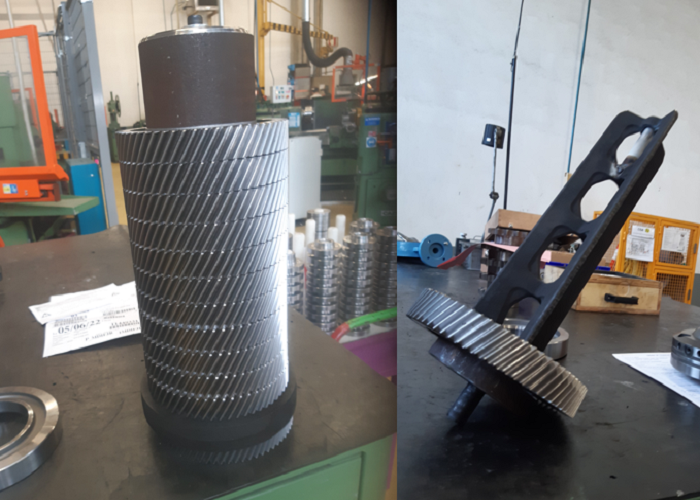
\includegraphics[width = 0.5\textwidth]{Figures/Cap3/Ensaio_simples.png}
    \caption[Montagem do ensaio do protótipo inicial da ferramenta modificada]%
    {Fotografia da montagem da ferramenta porta-peças modificada para o ensaio inicial da proteção do diâmetro.}
    \label{fig:ensaio_simples}
\end{figure}
%%%%%%%%%%%%%%%%%%%%%%%%%%%%%%%%%%%%%%%%%%%%%%%%%%%%%%%%%%%%%%%%%%%%%%%%%%%%%
%%%%%%%%%%%%%%%%%%%%%%%%%%%%%%%%%%%%%%%%%%%%%%%%%%%%%%%%%%%%%%%%%%%%%%%%%%%%%
\begin{figure}[htb!]
    \centering
    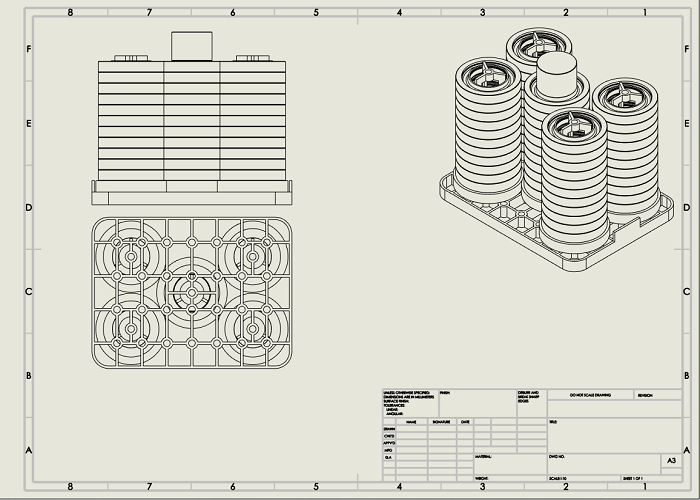
\includegraphics[width = 0.5\textwidth]{Figures/Cap3/Desenho_ensaio_simples.png}
    \caption[Desenho do esquema de montagem da ferramenta]%
    {Desenho feito em SolidWorks do esquema que foi montado o primeiro prato da carga de ensaio, onde a ferramenta modificada encontra-se no centro do primeiro prato da carga.}
    \label{fig:esquema_ensaio_simples}
\end{figure}
%%%%%%%%%%%%%%%%%%%%%%%%%%%%%%%%%%%%%%%%%%%%%%%%%%%%%%%%%%%%%%%%%%%%%%%%%%%%%
\newpage
\par
Para a realização das medições de dureza no Laboratório de Ensaios Mecânicos (LEMM) foram removidas as rodas de coroa de baixo, ou Nº 1, do meio, ou Nº 6 e de cima, ou Nº 10. Foram feitas filiações das duas zonas de soldadura do diferencial, denominadas por “Zona 1” e “Zona 2”; das duas zonas de prensagem, denominadas por “Zona 3” e “Zona 4”; das duas zonas de soldadura da “Cible”, denominadas por “Zona Cible 1” e “Zona Cible 2”; tres picagens nas zonas do dentado; e a dureza superficial, medida em HRC. A Figura \ref{fig:zonas_filiacoes_dureza} ilustra, num desenho de uma roda de coroa DB45, a posição das zonas das filiações de dureza.
%%%%%%%%%%%%%%%%%%%%%%%%%%%%%%%%%%%%%%%%%%%%%%%%%%%%%%%%%%%%%%%%%%%%%%%%%%%%%
\begin{figure}[htb!]
    \centering
    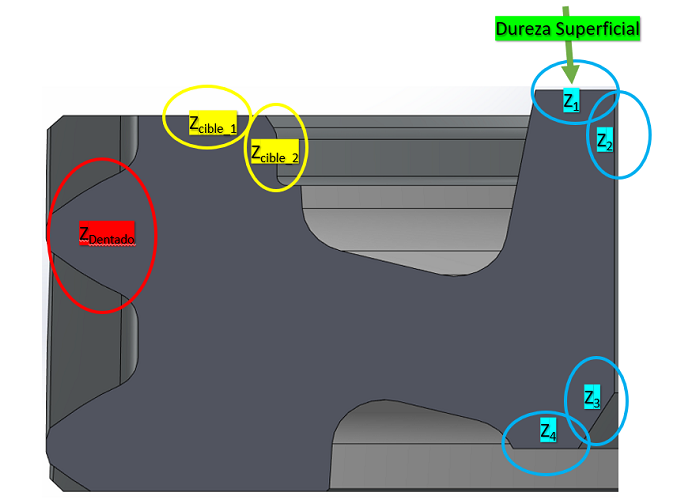
\includegraphics[width = 0.5\textwidth]{Figures/Cap3/Zonas_dureza.png}
    \caption[Zonas das filiações de dureza]%
    {Desenho indicativo das zonas onde são feitas as filiações de dureza das rodas de coroa, de forma a verificar se a proteção do diâmetro interno é efetiva e que nao há alterações nos valores de dureza do dentado.}
    \label{fig:zonas_filiacoes_dureza}
\end{figure}
%%%%%%%%%%%%%%%%%%%%%%%%%%%%%%%%%%%%%%%%%%%%%%%%%%%%%%%%%%%%%%%%%%%%%%%%%%%%%
\par
Os resultados destas filiações de dureza serão discutidos no Capítulo \ref{ch:resultados}, no entanto, para efeitos da continuidade do trabalho, é necessário dizer que, mesmo que os resultados tenham sido satisfatórios, os valores das durezas em todas as zonas nas rodas de coroa inferiores foram consideravelmente superiores aos valores nas rodas de coroa do meio e de cima. Além disso, na roda de coroa Nº 10, a dureza na zona de soldadura da Cible não foi afetada pela proteção, além da “zona 1” ter durezas ligeiramente superiores às durezas na mesma zona nas outras rodas de coroa, o que leva à suspeita de que a existência de uma aba seria necessária para uniformizar os valores de durezas em todas as 10 rodas de coroa da coluna. Por fim, verificou-se que a soldadura feita na falsa coroa à torre da ferramenta porta-peças sofreu rotura, o que também pode explicar o motivo das durezas em todas as zonas da roda de coroa Nº 1 serem muito maiores que as demais.
%%%%%%%%%%%%%%%%%%%%%%%%%%%%%%%%%%%%%%%%%%%%%%%%%%%%%%%%%%%%%%%%%%%%%%%%%%%%%
\subsection{Novos protótipos e melhorias} \label{ssec:novos_prototipos}
Devido aos problemas encontrados no ensaio do protótipo inicial, foram desenvolvidos dois outros protótipos. O primeiro, denominado “Tampa O” sendo uma modificação do protótipo inicial, apenas com a adição de uma aba de proteção para a cible. O segundo, alterando a geometria de um “copo” para um formato ajustado à torre da ferramenta porta-peças das peças de série, denominado “Tampa Y”. A Figura \ref{fig:novos_prototipos} ilustra as geometrias novas. A ferramenta inicial foi então denominada “Tampa P”, em homenagem ao “Engenheiro Pinto” responsável pela sua geometria e pela ideia de proteger o diâmetro interno das rodas de coroa quanto à Têmpera.
%%%%%%%%%%%%%%%%%%%%%%%%%%%%%%%%%%%%%%%%%%%%%%%%%%%%%%%%%%%%%%%%%%%%%%%%%%%%%
\begin{figure}[htb]
    \centering
    \begin{subfigure}{.5\textwidth}\
        \centering
        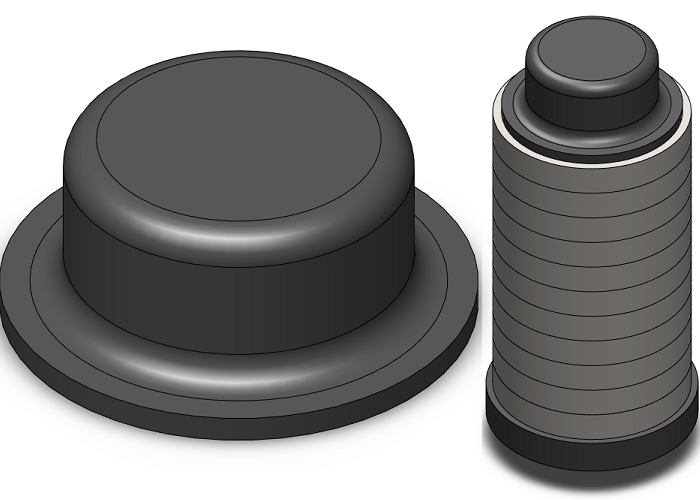
\includegraphics[width = 0.9\textwidth]{Figures/Cap3/Tampa_O.png}
        \caption{}  
    \end{subfigure}%
    \begin{subfigure}{.5\textwidth}
        \centering
        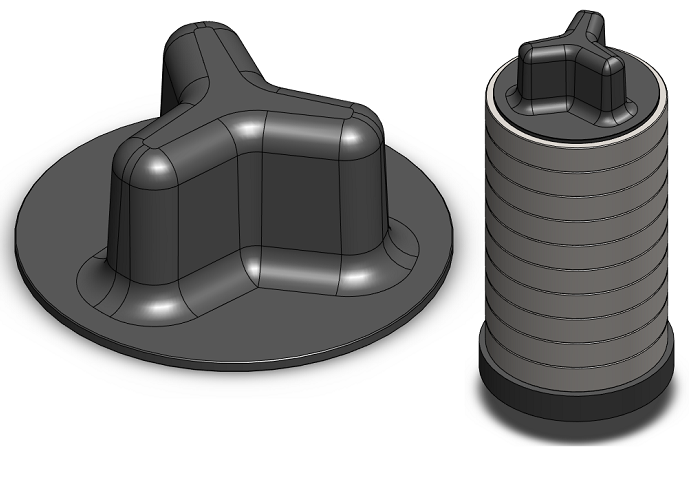
\includegraphics[width = 0.9\textwidth]{Figures/Cap3/Tampa_Y.png}
        \caption{}
    \end{subfigure}
    \caption[Modelos CAD dos novos protótipos de tampa]%
    {Modelos em CAD 3D dos novos protótipos que buscam melhorar os parâmetros resultantes do ensaio com a ferramenta inicial. À direita a “Tampa O” e à esquerda a “Tampa Y”.}
    \label{fig:novos_prototipos}
\end{figure}
%%%%%%%%%%%%%%%%%%%%%%%%%%%%%%%%%%%%%%%%%%%%%%%%%%%%%%%%%%%%%%%%%%%%%%%%%%%%%
\newpage
\par
Além da modificação das tampas, também foi modificada a junção da falsa coroa com a torre, uma vez que no protótipo inicial foi realizada uma soldadura muito simples, com apenas três “pingos” de soldadura em todo o diâmetro, desta vez, foi feita uma soldadura completa, em toda o diâmetro. Sendo as suspeitas de que os resultados do ensaio inicial foram afetados pela rotura da soldadura verdade, os próximos ensaios devem conferir resultados mais uniformes em todas as rodas de coroa da coluna tratada. Por fim, um novo protótipo foi testado para verificar a necessidade da utilização de uma tampa, sendo assim o próximo ensaio constituído por 5 colunas completas; uma coluna protegida pela tampa Y; uma coluna protegida pela tampa O; uma coluna protegida pela tampa P; uma coluna protegida apenas pela falsa coroa modificada, em baixo; e uma coluna sem proteção alguma, denominada coluna de série. Um desenho com o esquema de configuração deste prato para ensaio pode ser visto na Figura \ref{fig:configuracao_ensaio}.
%%%%%%%%%%%%%%%%%%%%%%%%%%%%%%%%%%%%%%%%%%%%%%%%%%%%%%%%%%%%%%%%%%%%%%%%%%%%%
\begin{figure}[htb!]
    \centering
    \begin{subfigure}{.5\textwidth}\
        \centering
        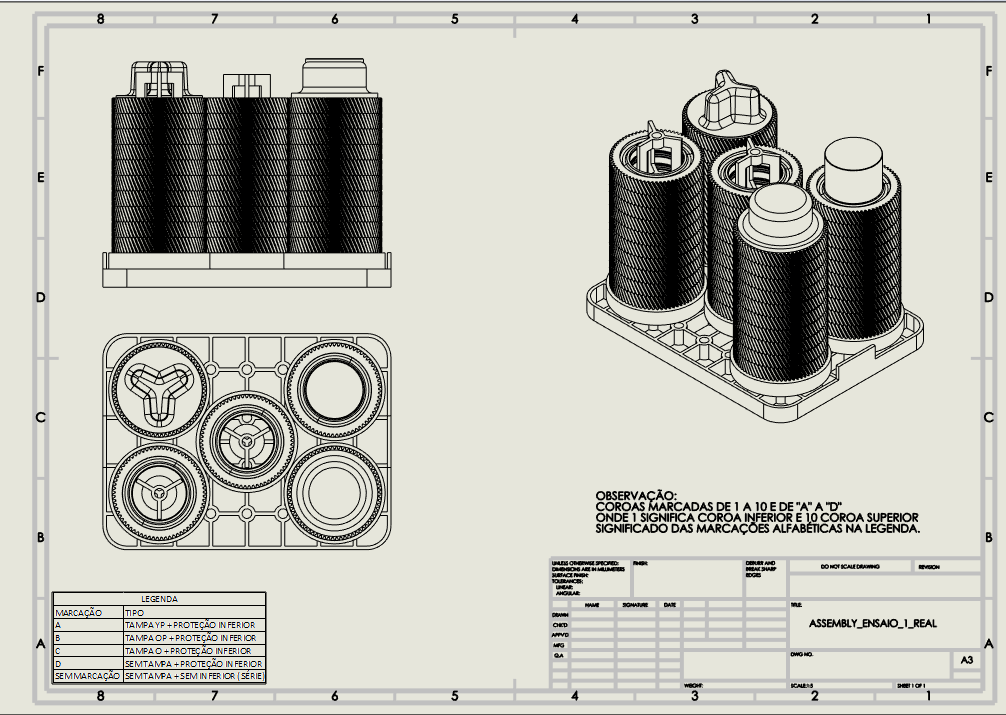
\includegraphics[width = 0.9\textwidth]{Figures/Cap3/Esquema_Prato_Ensaio_08-05-2023.png}
        \caption{}  
    \end{subfigure}%
    \begin{subfigure}{.5\textwidth}\
        \centering
        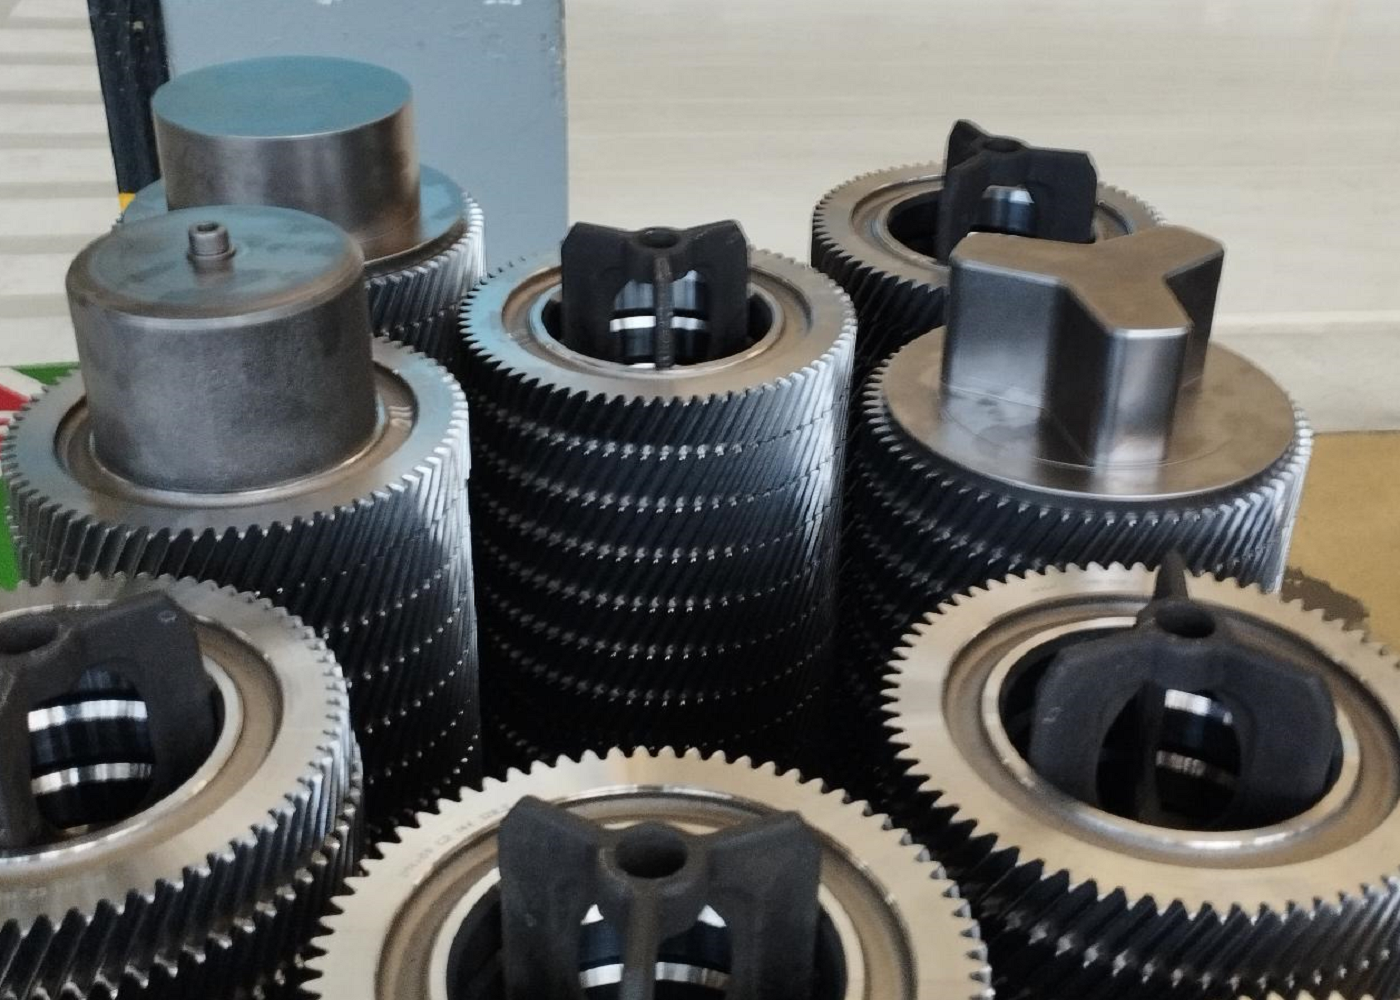
\includegraphics[width = 0.9\textwidth]{Figures/Cap3/Ensaio_varias_tampas.png}
        \caption{}  
    \end{subfigure}%
    \caption[Configuração do ensaio dos vários protótipos]%
    {à esquerda, um desenho indicativo da configuração das ferramentas num prato para realização do ensaio com os vários protótipos. À direita, uma fotografia da carga montada para ensaio.}
    \label{fig:configuracao_ensaio}
\end{figure}
%%%%%%%%%%%%%%%%%%%%%%%%%%%%%%%%%%%%%%%%%%%%%%%%%%%%%%%%%%%%%%%%%%%%%%%%%%%%%
\newpage
\par
Para a execução deste ensaio, foi necessário proceder à marcação das rodas de coroa, não só numa sequência numérica de 1 a 10, mas também numa sequência alfabética. Neste sistema, as rodas de coroa designadas por “A” correspondem à tampa Y, as “B” à tampa O, as “C” à tampa P, as “D” à coluna sem tampa, e as “S” à coluna de série. Assim, a roda de coroa marcada como “B10” representa, por exemplo, a roda de coroa no topo da coluna protegida pela tampa O. No ensaio anterior, surgiu um problema no reconhecimento das peças à entrada do forno de revenido, uma vez que o sistema se baseia na imagem do perfil do diâmetro da peça central, e as tampas não são identificadas automaticamente. Para contornar esta questão, optou-se por remover as tampas após a primeira máquina de lavar, tendo em conta que, caso fossem removidas após a têmpera, as tampas estariam a uma temperatura de 170\textdegree C, demasiado quente para uma manipulação segura.
\par
Paralelamente a este ensaio, realizou-se um segundo, com as mesmas configurações, mas desta vez utilizando rodas de coroa JT4. Foram adicionados dois provetes do material 27MC5, um no interior da coluna com geometria protegida pela tampa Y e outro no interior da coluna de série. Estes provetes foram posteriormente enviados para um laboratório em França, onde se procedeu à realização de uma espectroscopia de emissão ótica de descarga luminescente. Este ensaio tem como objetivo aferir a composição dos materiais constituintes no provete, em particular, verificar a ocorrência de enriquecimento de carbono e azoto no diâmetro interno das rodas de coroa protegidas no forno de carbonitruração, e comparar os resultados com o enriquecimento observado nas rodas de coroa de série. Um esquema do ensaio e a posição dos provetes estão ilustrados na Figura \ref{fig:ensaio_gales}. Uma fotografia de um provete antes do ensaio pode ser observada na Figura \ref{fig:gales}.
%%%%%%%%%%%%%%%%%%%%%%%%%%%%%%%%%%%%%%%%%%%%%%%%%%%%%%%%%%%%%%%%%%%%%%%%%%%%%
\begin{figure}[htb!]
    \centering
    \begin{subfigure}{.5\textwidth}\
        \centering
        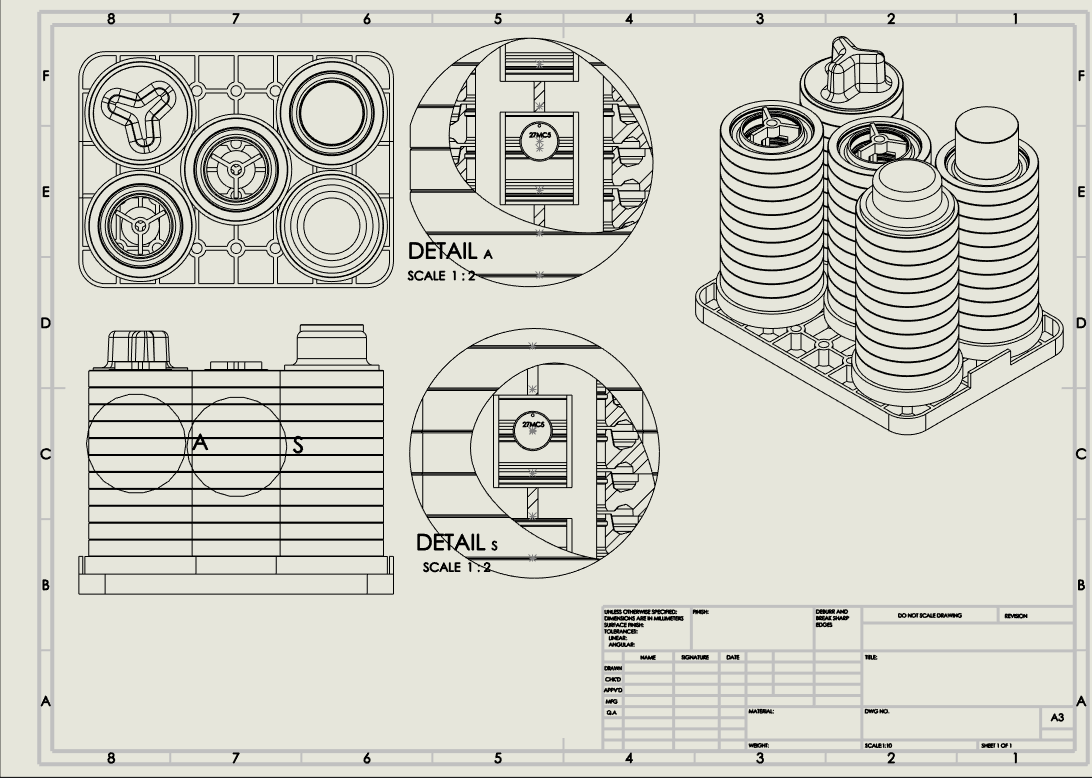
\includegraphics[width = 0.9\textwidth]{Figures/Cap3/Layout_ensaio_gallets.png}
        \caption{}
        \label{fig:ensaio_gales}  
    \end{subfigure}%
    \begin{subfigure}{.5\textwidth}\
        \centering
        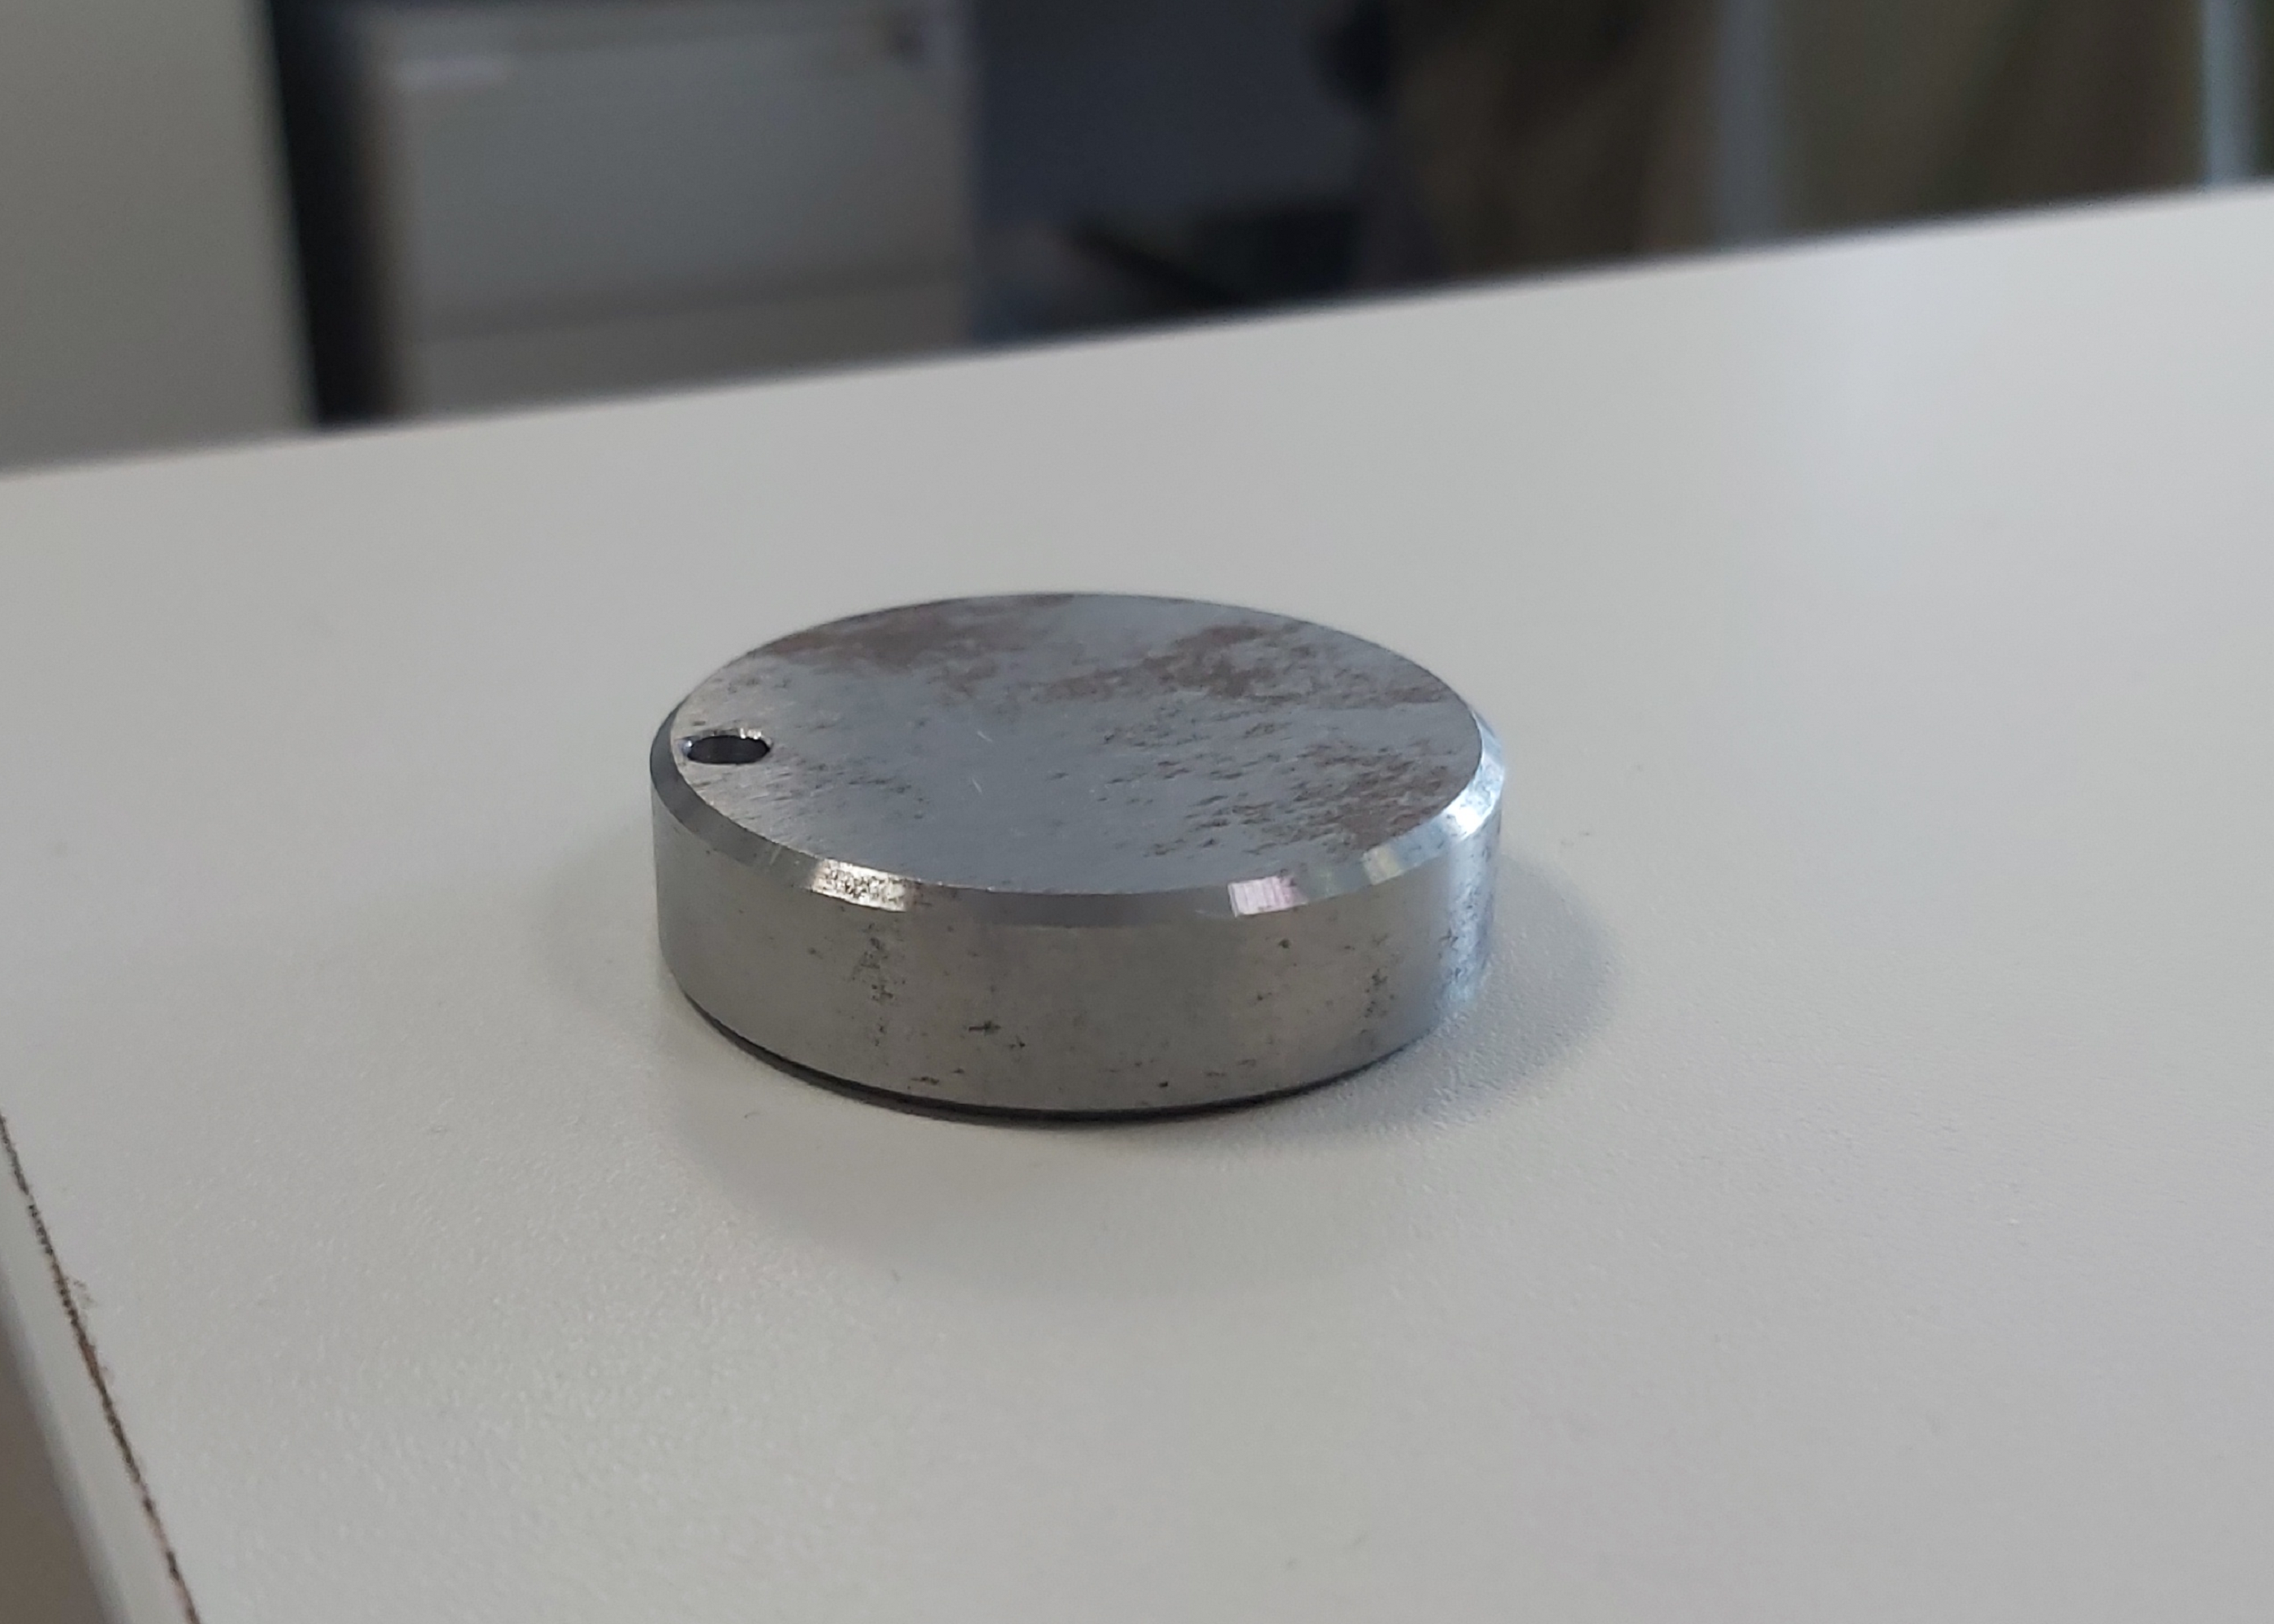
\includegraphics[width = 0.9\textwidth]{Figures/Cap3/Gallets.png}
        \caption{}
        \label{fig:gales}  
    \end{subfigure}%
    \caption[Configuração do ensaio dos vários protótipos]%
    {à esquerda, desenho indicativo da configuração das ferramentas num prato para realização do ensaio com os vários protótipos. Esta configuração é idêntica ao ensaio anterior, com a adição de duas galés, uma por dentro da coluna protegida por tampa Y, e uma por dentro da coluna de série. À direita, fotografia de uma das galés que foram inseridas na carga de ensaio.}
\end{figure}
%%%%%%%%%%%%%%%%%%%%%%%%%%%%%%%%%%%%%%%%%%%%%%%%%%%%%%%%%%%%%%%%%%%%%%%%%%%%%
\newpage
\par
Após este último, procedeu-se a um novo ensaio, desta vez com as rodas de coroa DB35, mantendo a mesma configuração dos ensaios anteriores realizados com as rodas de coroa DB45 e JT4. No entanto, tendo em conta que o tratamento e a recolha dos valores de dureza de cada ensaio demoram aproximadamente duas semanas para serem completados, à data da redação deste documento, os resultados ainda não estavam disponíveis. Consequentemente, o tratamento e a análise dos dados deste último ensaio não serão abordados no capítulo seguinte. Estava igualmente prevista a realização de um ensaio utilizando uma tinta "stop-off carbonitruração", bem como um ensaio no forno de revenido para a verificação do hidrogénio difusível. Infelizmente, devido ao escasso tempo disponível, estes ensaios não puderam ser realizados.
%%%%%%%%%%%%%%%%%%%%%%%%%%%%%%%%%%%%%%%%%%%%%%%%%%%%%%%%%%%%%%%%%%%%%%%%%%%%%
\subsection{Parâmetros de Conformidade e Metodologia de Ensaio} \label{ssec:parametros_metodologia}
Por fim, é importante elucidar o intervalo de parâmetros desejados para as rodas de coroa, bem como a metodologia de ensaio empregada para aferir tais parâmetros de conformidade. Importa ainda salientar que, caso estes parâmetros não sejam verificados na roda de coroa em teste, que nas rodas de coroa de série corresponde sempre à roda superior da coluna central do prato do meio de uma carga, toda a carga deve ser rejeitada e, por consequência, tratada como sucata. A Tabela \ref{tab:parametros_conformidade} apresenta os valores correspondentes aos diversos pontos, sendo estes os mesmos para todas as séries de roda de coroa, nomeadamente JT4, DB35 e DB45.
%%%%%%%%%%%%%%%%%%%%%%%%%%%%%%%%%%%%%%%%%%%%%%%%%%%%%%%%%%%%%%%%%%%%%%%%%%%%%
\begin{table}
    \centering
    \refstepcounter{table}
    \caption[Parâmetros de conformidade para rodas de coroa]%
    {Valores dos intervalos dos parâmetros de conformidade para rodas de coroa JT4, DB35 e DB45.}
    \label{tab:parametros_conformidade}
    \begin{tabular}{llr} 
    \toprule
    \multicolumn{1}{c}{\textbf{Etapa}} & \multicolumn{1}{c}{\textbf{Parâmetro de conformidade}} & \multicolumn{1}{c}{\textbf{Intervalo}}  \\ 
    \hline\hline
    \multirow{4}{*}{Peça Branca}       & Dentado sem riscos ou lascas                           & Sem defeito visual                      \\
                                       & Diâmetro externo                                       & 120,00 ± 0,04 mm                        \\
                                       & Diâmetro interno                                       & 80,00 ± 0,04 mm                         \\
                                       & Altura da peça                                         & 50,00 ± 0,04 mm                         \\ 
    \hline
    \multirow{4}{*}{Peça Negra}        & Dureza do dentado                                      & 680 a 900 HV                            \\
                                       & EC650                                                  & 0,6 a 0,8 mm                            \\
                                       & ET                                                     & 0,8 a 1,2 mm                            \\
                                       & Austenite residual                                     & Até 40\%                                \\
    \bottomrule
    \end{tabular}
\end{table}
%%%%%%%%%%%%%%%%%%%%%%%%%%%%%%%%%%%%%%%%%%%%%%%%%%%%%%%%%%%%%%%%%%%%%%%%%%%%%